\documentclass[10pt,fleqn,xcolor=dvipsnames]{beamer}
\beamertemplatenavigationsymbolsempty
\usetheme{Boadilla}
\DeclareGraphicsExtensions{.jpg,.eps,.png,.pdf,.mps,.gif}
\usepackage[latin1]{inputenc}
\usepackage[T1]{fontenc}
\usepackage[english]{babel}
\usepackage{pgf,pgfarrows,pgfnodes,pgfautomata,pgfheaps}
\usepackage{amsmath}
\usepackage{amsfonts}
\usepackage{graphicx}
\usepackage{color}
\usepackage{lmodern}
\usepackage[3D]{movie15}
\usepackage{algorithm}
\usepackage{algpseudocode}
\usepackage{url}
\usepackage{placeins}
\usepackage{textcmds}
\usepackage{listings}

\colorlet{grey}{gray!40}
\definecolor{PG}{rgb}{0.0, 0.27, 0.13}
%%%%%%%%%%%%%%%%%%%%%%%%%%%%%%%%%%%%%%%%%%%%%%%%%%%%%%%%%%%%%%%%%%%%%%%%%%%%%%%%%%%%%%%
% title page definition %%%%%%%%%%%%%%%%%%%%%%%%%%%%%%%%%%%%%%%%%%%%%%%%%%%%%%%%%%%%%%%
%%%%%%%%%%%%%%%%%%%%%%%%%%%%%%%%%%%%%%%%%%%%%%%%%%%%%%%%%%%%%%%%%%%%%%%%%%%%%%%%%%%%%%%
\setbeamercovered{dynamic}
\setbeamerfont{author}{family=\rmfamily}
\author[M. Beccuti,   R. J. P. Bonnal
and  R. Calogero]{\large{\textbf{M. Beccuti,  R. J. P. Bonnal
 and R. Calogero}}\\[15pt]\emph{Universit\`{a} degli Studi di Torino \\  Istituto Nazionale di Genetica Molecolare \qq{Romeo ed Enrica Invernizzi}
}\\~\\~ \textbf{ELIXIR-IIB Training Platform}~\\\tiny(First day)}
\title[Docker and Reproducibility]{\Large{\textbf{Docker and Reproducibility}}}
%\institute{\normalsize{} \\
%\footnotesize{Boston Park Plaza Hotel, Boston, Massachusetts USA}}
\date[June 2019]{June 2019}
\titlegraphic{
\begin{flushright}

\includegraphics[height=2cm]{Figure/LogoTorino}
\includegraphics[height=2cm]{Figure/LogoINGM_original}
\end{flushright}
}

% table of contents depth
\setcounter{tocdepth}{1}
\begin{document}
\usebackgroundtemplate{
\includegraphics[width=140mm]{Figure/BackgroundTorino}}
\setcounter{tocdepth}{5}
%#Frame 1 title
\frame[plain]{\titlepage}


\frame{
  \frametitle{Outline}  \vspace{0.3cm}
    \begin{block}{Training aims:}
\begin{itemize}
\item Create and run  a docker image; 
\item Develop a  docker service;
\end{itemize}    
\end{block}
}
\frame{
\frametitle{Outline} \vspace{0.3cm}
 \vspace{0.5cm}
\begin{enumerate}
\item Introduction\vspace{0.2cm}
\begin{itemize}
\item Virtualization: Virtual Machines and containers; \vspace{0.2cm}
\item Containers in Linux: Docker project; \vspace{0.2cm}
\end{itemize}
\item Command Line Interface
\item A simple example: how to embed an application in a Docker Image; \vspace{0.2cm}
\begin{itemize}
\item DockerHub
\item Volumes: sharing data with the containers
\item Building a Docker Image with R
\end{itemize}
\item Automate Docker Image building\vspace{0.2cm}
\begin{itemize}
\item scripting the build of an Image
\item building a custom Image using a dockerfile
\item dockerfile best practices
\end{itemize}
\end{enumerate}
  }

    
  
  \frame{
  \frametitle{What are \emph{containers} and \emph{Virtual Machines}?}
  \begin{columns}[T] % align columns
  \begin{column}{.80\textwidth}
  	\begin{itemize}
   		\item Containers and Virtual Machines (VM) are similar in their goals: 
\begin{enumerate}   		
   		\item \emph{\color{NavyBlue}to provide analysis \textbf{portability} isolating an application  into a self-contained unit that can run anywhere};\vspace{0.3cm}
   		\item \emph{\color{NavyBlue}to provide analysis \textbf{reproducibility} freezing the version of  tools and libraries used.}
   		\end{enumerate}
   		\vspace{0.3cm}
   		\item  They remove the need for physical hardware, allowing for more efficient use of computing resources, both in terms of energy consumption and cost effectiveness;\vspace{0.3cm}
   		\item 	The main difference between containers and VMs is in their architectural approach.
   		\end{itemize}\vspace{0.3cm}
   \end{column}%
   \hfill%
   \begin{column}{0.20\textwidth}
     	\begin{center}
  			
\includegraphics[width=1.15\columnwidth]{./Figure/DockerVSVM}\\
  		\end{center}
   \end{column}%
   \end{columns}
  } 



 \frame{
  \frametitle {Virtual Machines}
  
  \begin{columns}[T] % align columns
  \begin{column}{.55\textwidth}
  	\begin{itemize}
 		\item A VM is essentially an emulation of a real computer (i.e.\emph{ \color{NavyBlue} guest machine}) that executes programs like a real computer;\vspace{0.3cm}
 
 		\item  VMs run on top of a physical machine (i.e.\emph{\color{NavyBlue} host machine}) using a \emph{\color{NavyBlue}hypervisor};\vspace{0.3cm}
 
 		\item A {\color{NavyBlue}hypervisor} is a piece of software, firmware, or hardware;\vspace{0.3cm}
 		
 		\item A {\color{NavyBlue}guest machine} contains:
		
		\begin{itemize}	 		
 		
 		 \item both the application and whatever it needs to run that application (e.g. system binaries and libraries). 
 	
 	    \item a virtualized hardware stack including virtualized network adapters, storage, CPU \dots.
 	
 		\end{itemize}
 		
      	\end{itemize}
   \end{column}%
   \hfill%
   \begin{column}{0.45\textwidth}
     	\begin{center}
  			\includegraphics[width=1.00\columnwidth]{./Figure/VM}\\
  		\end{center}
   \end{column}%
   \end{columns}
  } 
  
  
  
  
  \frame{
  \frametitle {Containers}
  
  \begin{columns}[T] % align columns
  \begin{column}{.55\textwidth}
  	\begin{itemize}
 		\item Unlike a VM which provides hardware virtualization, a container provides operating-system-level virtualization by abstracting the \emph{\color{NavyBlue} user space};\vspace{0.3cm}
 
 		\item The main difference between containers and VMs is that containers \textbf{share} the host system's kernel with other containers.\vspace{0.3cm}
 
      	\end{itemize}
   \end{column}%
   \hfill%
   \begin{column}{0.45\textwidth}
     	\begin{center}
  			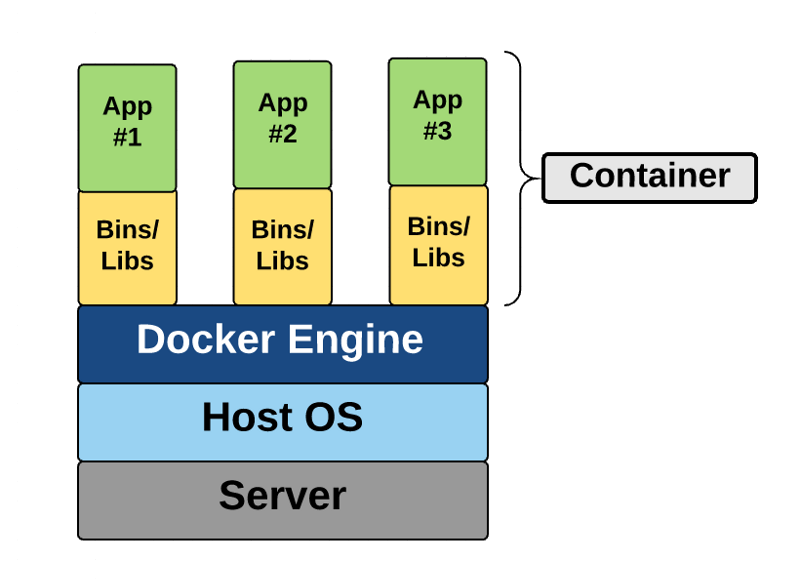
\includegraphics[width=1.05\columnwidth]{./Figure/Container}\\
  		\end{center}
   \end{column}%
   \end{columns}
  } 
  

 \frame{
  \frametitle {Containers VS VM}
  
  \begin{columns}[T] % align columns
  \begin{column}{.50\textwidth}
		\begin{center}
  			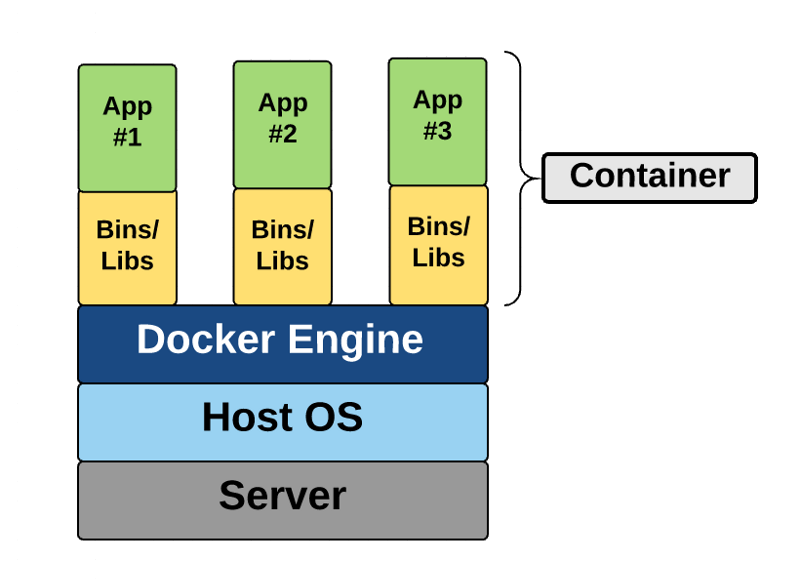
\includegraphics[width=1.00\columnwidth]{./Figure/Container}\\
  		\end{center}
   \end{column}%
   \hfill%
   \begin{column}{0.50\textwidth}
     	\begin{center}
  			\includegraphics[width=1.00\columnwidth]{./Figure/VM}\\
  		\end{center}
   \end{column}%
   \end{columns}
  } 

\frame{
  \frametitle {Containers VS VM}
 	\begin{center}
  			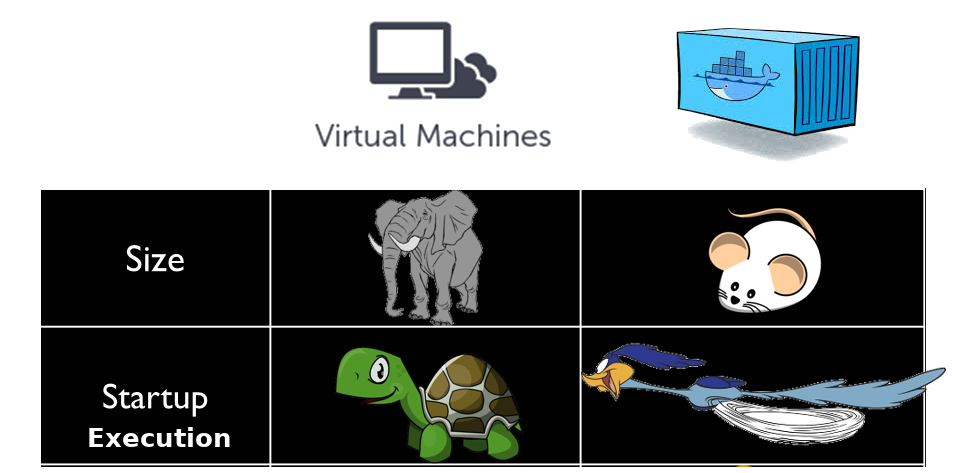
\includegraphics[width=0.90\columnwidth]{./Figure/ContainersVSVM}\\
  		\end{center}
  } 

\frame{
\frametitle{Docker container, VM and real server: a comparison}
In [1] a comparison among physical server, KVM, and Docker is reported.

     	\begin{center}
  			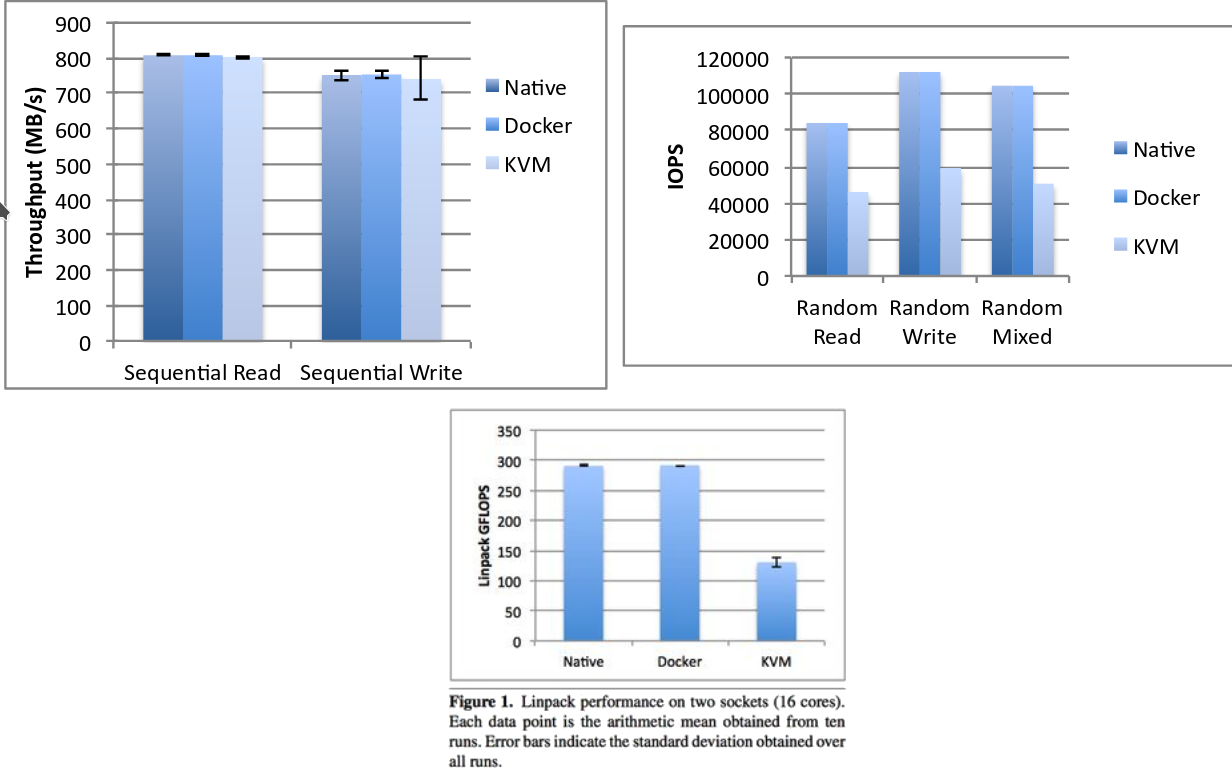
\includegraphics[width=0.90\columnwidth]{./Figure/benchmark}
  		\end{center}  
{\tiny
[1] W. Felter, A. Ferreira, R. Rajamony and J. Rubio, \emph{\textbf{An updated performance comparison of virtual machines and Linux containers}}, 2015 IEEE International Symposium on Performance Analysis of Systems and Software (ISPASS), Philadelphia, PA, 2015, pp. 171-172.

}
} 



\frame{
\frametitle{Computational Reproducibility Stack}

       	\begin{center}
  			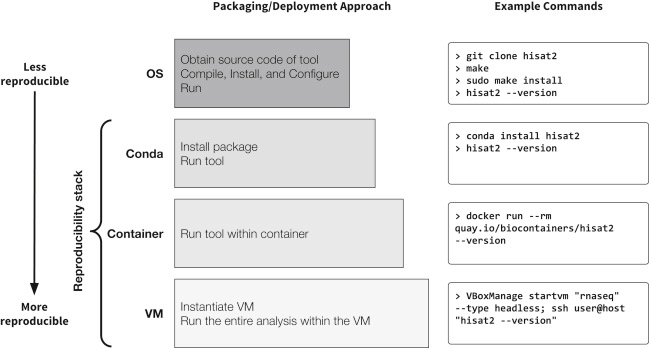
\includegraphics[width=0.9\columnwidth]{./Figure/stack}\\
  		\end{center}
}

 \frame{
  \frametitle {}
  \centerline{\Huge \color{NavyBlue} \textbf{\emph{Docker project}}}
       	\begin{center}
  			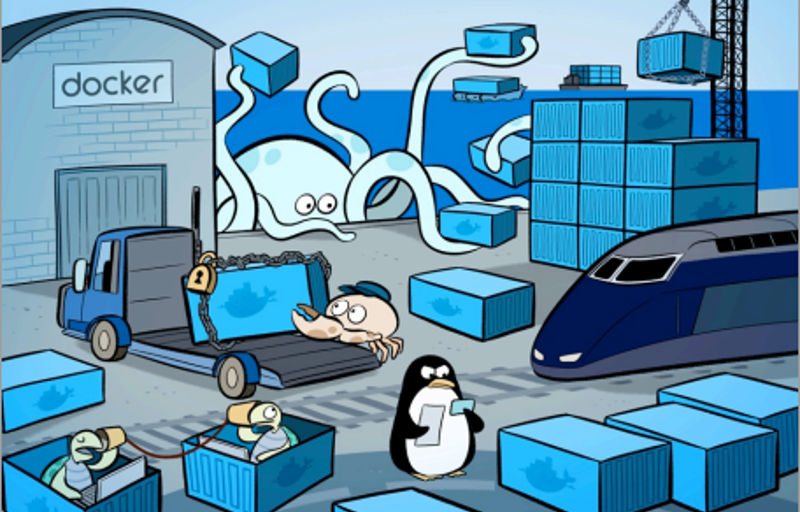
\includegraphics[width=0.8\columnwidth]{./Figure/basic}\\
  		\end{center}
}

  
  
 \frame{
  \frametitle {Docker project}
  
  
  
  \begin{columns}[T] % align columns
  \begin{column}{.55\textwidth}
  	\begin{itemize}
 		\item Docker is an open-source project based on Linux containers.
 	\vspace{0.3cm}
 		\item Others Linux container technologies include Solaris Zones, BSD jails, and LXC, which have been around for many years.
 		 	\vspace{0.3cm}	
      	\end{itemize}
   \end{column}%
   \hfill%
   \begin{column}{0.45\textwidth}
     	\begin{center}
  			
\includegraphics[width=1.05\columnwidth]{./Figure/Docker}\\
  		\end{center}
   \end{column}%
   \end{columns}
   \centerline{\Large \color{NavyBlue} \textbf{Why to use Docker??}}
  } 
  
  
  

 \frame{
  \frametitle {Why to use Docker?}
  
    \begin{columns}[T] % align columns
  \begin{column}{.65\textwidth}
  	\begin{itemize}
	\item  \textbf{\color{NavyBlue} Ease of use:} Docker has made it much easier for anyone to take advantage of containers in order to quickly build and test portable applications; \vspace{0.3cm}	
	
	\item  \textbf{\color{NavyBlue} Speed:} Docker containers are very lightweight and fast.
	\vspace{0.3cm}	
	\item \textbf{\color{NavyBlue}Docker Hub:} Docker users also benefit from the increasingly rich repository of Docker Hub, which you can think of as an "app store for Docker images"; 
	\vspace{0.3cm}	
	\item \textbf{\color{NavyBlue}Modularity and Scalability:} Docker makes it easy to break out your application's functionality into individual containers.
  	\end{itemize}
   \end{column}%
   \hfill%
   \begin{column}{0.35\textwidth}
     	\begin{center}
  			
\includegraphics[width=1.05\columnwidth]{./Figure/Docker}\\
  		\end{center}
   \end{column}%
   \end{columns}
  } 
    
  

  \frame{
\frametitle{Docker basics} 
\vspace{0.2cm}
\begin{itemize}
\item \textbf{\color{NavyBlue}\emph{Image}} is an executable package that includes everything needed to run an application (i.e. its code,  libraries, environment variables, and configuration files);\vspace{0.2cm}
\item \textbf{\color{NavyBlue}\emph{Container}} is a run-time instance of an image;\vspace{0.2cm}
\item \textbf{\color{NavyBlue}\emph{Volume}} is used to  share files from the host machine to containers.
\end{itemize}
\vspace{0.2cm}
  \begin{center}
  			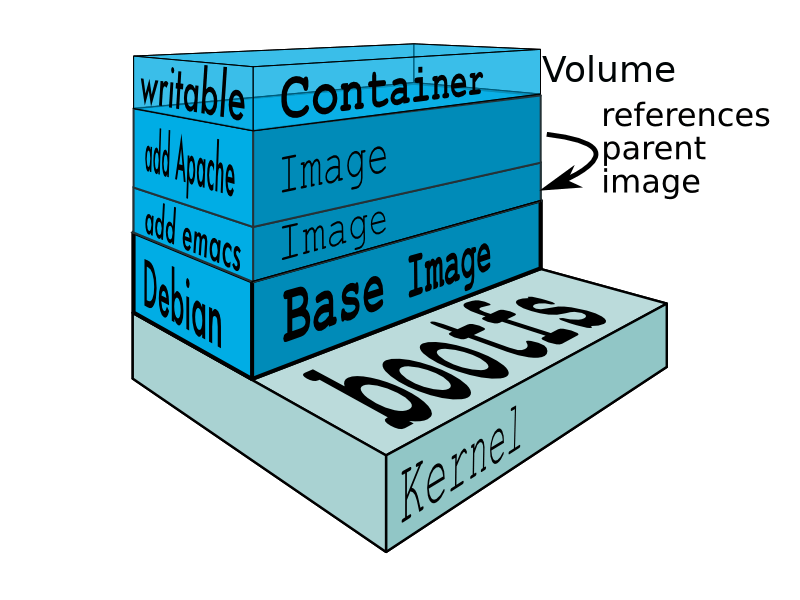
\includegraphics[width=0.55\columnwidth]{./Figure/exec}\\
  		\end{center} 

}

 \frame{
  \frametitle {Docker schema}
  
  
  
  \begin{columns}[T] % align columns
  \begin{column}{.55\textwidth}
  	\begin{itemize} 		
  	\item \textbf{\color{NavyBlue}Docker client:} provides an interface for users;
 	\vspace{0.2cm}
 		\item \textbf{\color{NavyBlue}Docker Host:} executes the commands sent to the Docker Client;\vspace{0.2cm}

 		\item \textbf{\color{NavyBlue}Docker Hub:} remove repository storing docker's images.
      	\end{itemize}
   \end{column}%
   \hfill%
   \begin{column}{0.45\textwidth}
     	\begin{center}
  			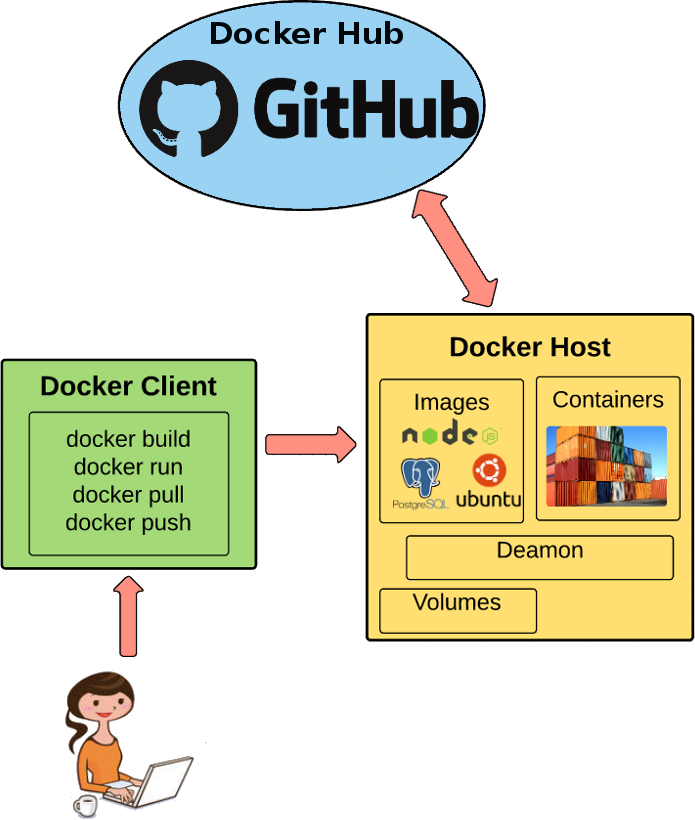
\includegraphics[width=0.95\columnwidth]{./Figure/DockerSchema}\\
  		\end{center}
   \end{column}%
   \end{columns}
  } 
  
  
  
   \frame{
  \frametitle {}
  \vspace{1.5cm}
  \centerline{\Huge \color{NavyBlue} \textbf{\emph{Create a docker image for }}}
  \centerline{\Huge \color{NavyBlue} \textbf{\emph{FastQC tool}}}
  \vspace{0.4cm}
     	\begin{center}
  			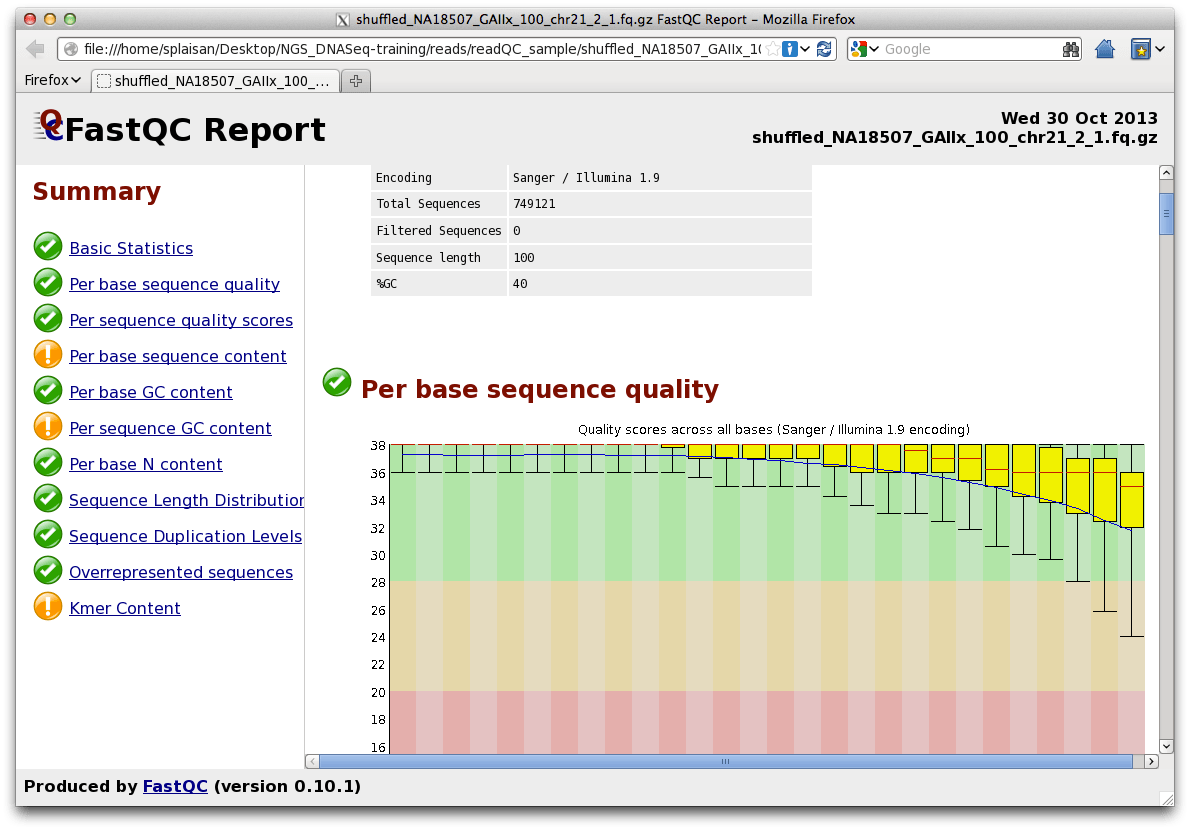
\includegraphics[width=0.60\columnwidth]{./Figure/FastQC}
  		\end{center} 

}

   \frame{
  \frametitle {Create a docker image for FastQC tool}
\vspace{0.4cm}
   \centerline{\color{NavyBlue} \textbf{\emph{FastQC in nutshell}}}\vspace{0.4cm}
   \begin{itemize}
   \item It is  quality control tool for high throughput sequence data;\vspace{0.2cm}
   \item It is written in Java;\vspace{0.2cm}
   \item It is main functions are:\vspace{0.1cm}
   \begin{itemize}
   \item Import of data from BAM, SAM or FastQ files (any variant);\vspace{0.1cm}
   \item Providing a quick overview to tell you in which areas there may be problems;\vspace{0.1cm}
   \item Summary graphs and tables to quickly assess your data;\vspace{0.1cm}
   \item Export of results to an HTML based permanent report;\vspace{0.1cm}
   \item Offline operation to allow automated generation of reports without running the interactive application.
   \end{itemize} 
   \end{itemize}     	
   \begin{center}
  			
\includegraphics[width=0.15\columnwidth]{./Figure/QC}
  		\end{center} 
  }
  
 \frame{
  \frametitle {Create a docker image for FastQC tool}
   \centerline{\color{NavyBlue} \textbf{\emph{How to create FastQC image}}}\vspace{0.4cm}
  \begin{itemize}
  \item Download and update a basic image (use Fedora);\vspace{0.2cm}
  \item Download and install \textbf{\color{NavyBlue}Oracle Java} on the download image;\vspace{0.2cm}
  \item Download and install  \textbf{\color{NavyBlue}unzip} on the download image;\vspace{0.2cm}
  \item Download and install  \textbf{\color{NavyBlue}perl} on the download image;\vspace{0.2cm}
  \item Download and install  \textbf{\color{NavyBlue}FastQC} on the download image;\vspace{0.2cm}
  \item Run the embedded FastQC on fastq data.
\end{itemize}     
  }

\frame{
  \frametitle {Download and update a basic image}
  \begin{itemize}
  	\item Download Fedora; 
  	          	\begin{center}
  			
\includegraphics[width=0.95\columnwidth]{./Figure/pullFedora}
  		\end{center}	
  		
  	 \end{itemize}	
  		}
  		
  		
 \frame{
  \frametitle {Download and update a basic image}
  \begin{itemize} 		
  	\item Create a new tag from Fedora image.
          	\begin{center}
  			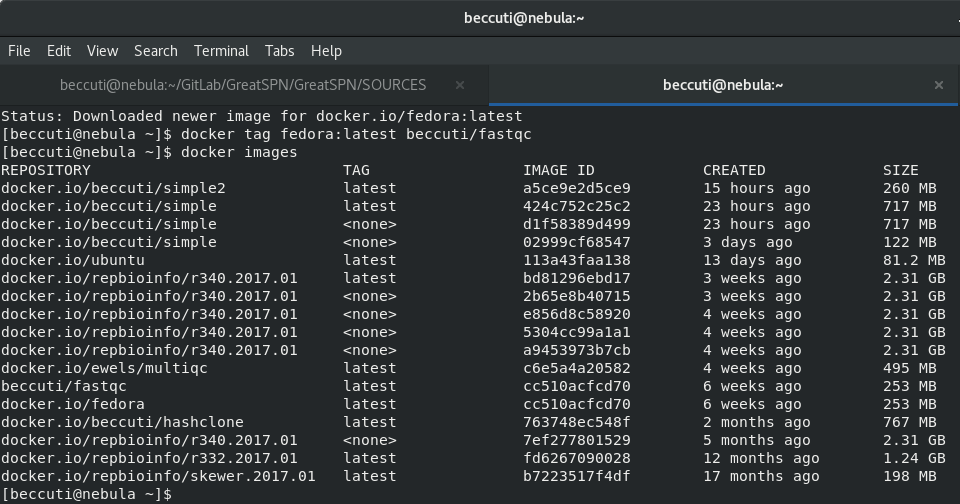
\includegraphics[width=0.95\columnwidth]{./Figure/tagFastQC}
  			\end{center}	
 \end{itemize}
} 
  	 
 \frame{
  \frametitle {Download and update a basic image}
  \begin{itemize} 		
  	\item Update Fedora using \emph{\color{PineGreen} dnf update};
          	\begin{center}
  			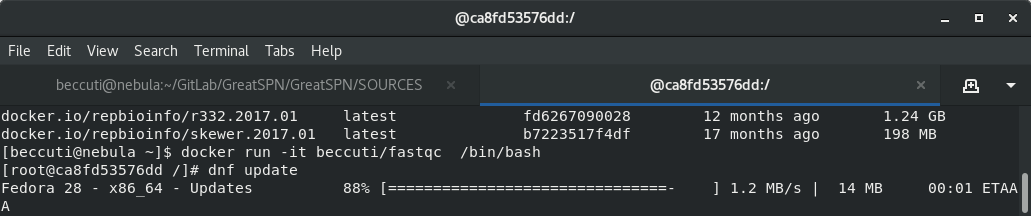
\includegraphics[width=0.95\columnwidth]{./Figure/updateFedora}
  			\end{center}	
   \item  Commit the updated image.
   		    \begin{center}
  			
\includegraphics[width=0.95\columnwidth]{./Figure/commitFedora}
  			\end{center}	
 \end{itemize}
} 
  	\frame{
  \frametitle {Download and install Oracle Java}
  \begin{itemize} 		
  	\item Download \textbf{\color{NavyBlue}Java RE ORACLE} (\url{http://www.oracle.com});\vspace{0.2cm}
  	\item Install  \textbf{\color{NavyBlue}Java RE ORACLE}
          	\begin{center}
  			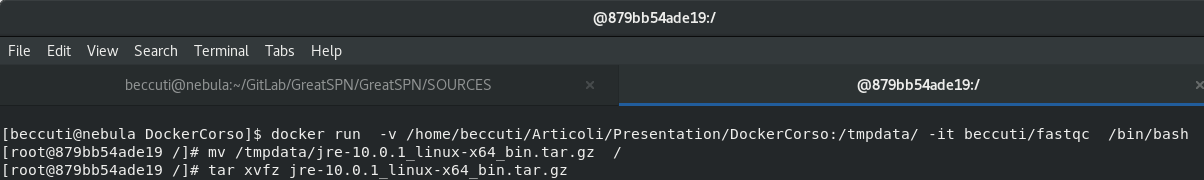
\includegraphics[width=0.95\columnwidth]{./Figure/javaFedora}\vspace{0.2cm}
  			\end{center}	
   \item  Create a symbolic link in \emph{bin} for java program.
   		    \begin{center}
  			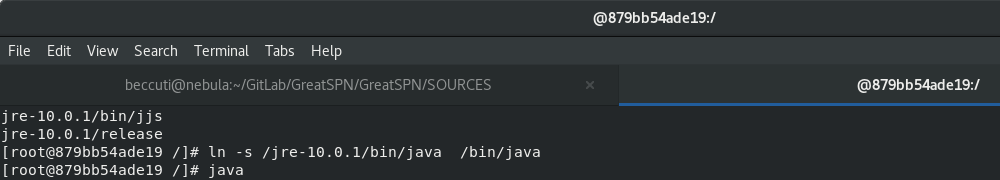
\includegraphics[width=0.95\columnwidth]{./Figure/javaFedora2}
  			\end{center}	
 \end{itemize}
}   	 
  
	\frame{
  \frametitle {Download and install FastQC}
  \begin{itemize} 		
  	\item Install \textbf{\color{NavyBlue} unzip} command using   \emph{\color{PineGreen} dnf install unzip.x86\_64};
          	\begin{center}
  			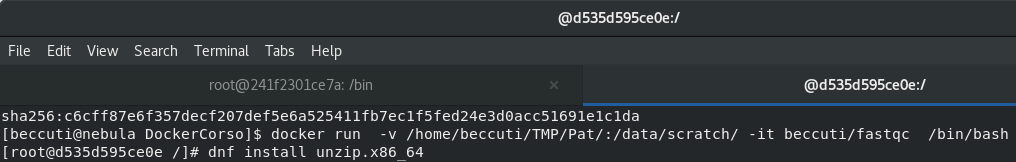
\includegraphics[width=0.95\columnwidth]{./Figure/unzipFedora}\vspace{0.2cm}
  			\end{center}		
  	\item Install  \textbf{\color{NavyBlue}perl} command using   \emph{\color{PineGreen} dnf install perl.x86\_64};
          	\begin{center}
  			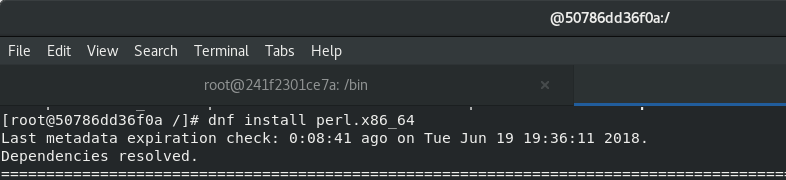
\includegraphics[width=0.95\columnwidth]{./Figure/perlFedora}\vspace{0.2cm}
  			\end{center}	
   \end{itemize}
} 			
  
  			
   
\frame{
  \frametitle {Download and install FastQC}
  \begin{itemize}  			
   \item Unzip  FastQC program;
   		    \begin{center}
  			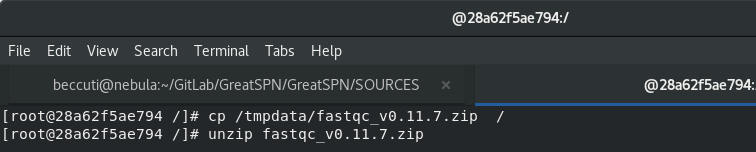
\includegraphics[width=0.95\columnwidth]{./Figure/fastqcFedora}
  			\end{center}	\vspace{0.1cm}
	\item Make FastQC program executable  and create a symbolic link in \emph{bin} for it;
	  	  		    \begin{center}
  			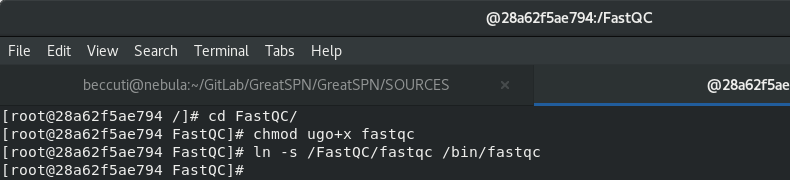
\includegraphics[width=0.95\columnwidth]{./Figure/fastqcFedora1}
  			\end{center}		\vspace{0.1cm}				
 \end{itemize}
}   	

\frame{
  \frametitle {Download and install FastQC}
  \begin{itemize}  			
 	\item Commit the updated image.
 	 	   \begin{center}
  			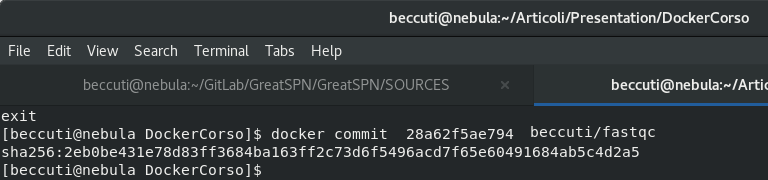
\includegraphics[width=0.95\columnwidth]{./Figure/fastqcFedora2}
  			\end{center}				
 \end{itemize}
}   	      
  	
 \frame{
  \frametitle { Download and install FastQC}
  \begin{itemize}  			
   \item  We use \textbf{\color{NavyBlue}gedit} to create our  bash script; \vspace{0.2cm}
   		    \begin{center}
  			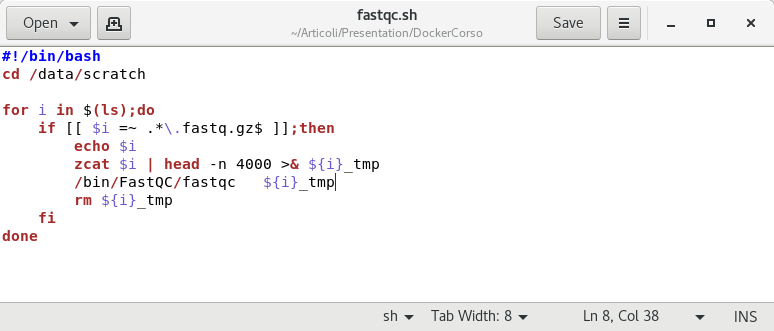
\includegraphics[width=0.95\columnwidth]{./Figure/fastqcGedit}
  			\end{center}	
  \end{itemize}
}   	    	  

 \frame{
  \frametitle { Download and install FastQC}
  \begin{itemize}   	  			
	\item Update the image adding the created script. \end{itemize}
	\vspace{0.2cm}
	  	  		    \begin{center}
  			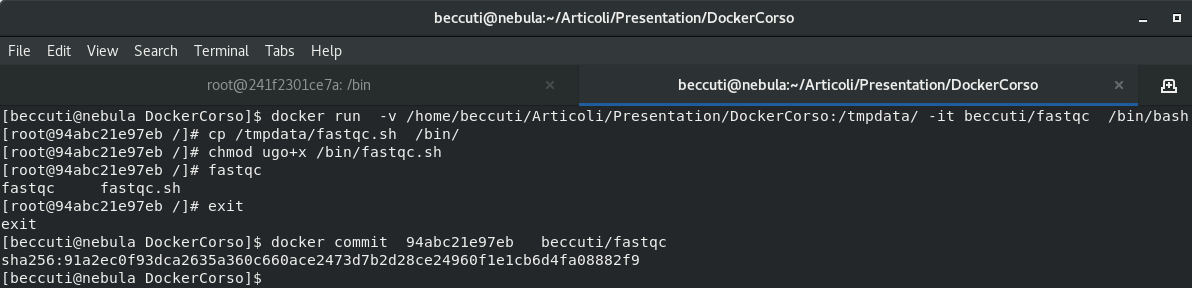
\includegraphics[width=1.0\columnwidth]{./Figure/fastqcshFedora}
  			\end{center}				

}  

 	    	  
 \frame{
  \frametitle {Run the embedded FastQC}
  \begin{itemize}   	  			
	\item Execute the embedded FastQC on .fastq files.\vspace{0.2cm}
	\item The folder containing .fastq files must be mount as /data/scratch  \end{itemize}
	
	  	    \begin{center}
  			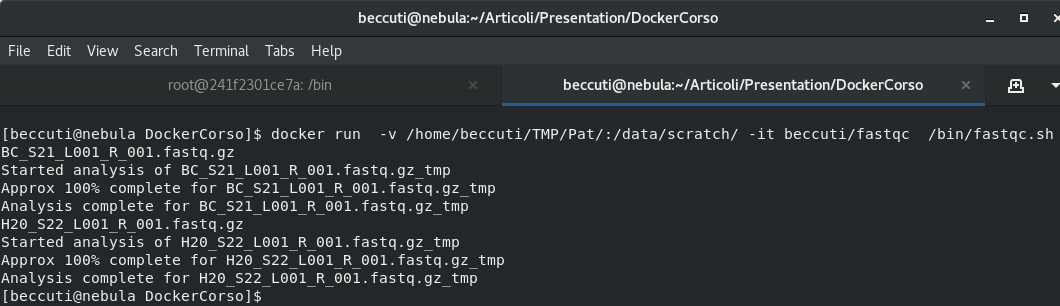
\includegraphics[width=1.0\columnwidth]{./Figure/fastqrunFedora}
  			\end{center}	
  						

}

 	    	  
 \frame{
  \frametitle {Run the embedded FastQC}
  \begin{itemize}   	  			
	\item FastQC output:
	  	    \begin{center}
  			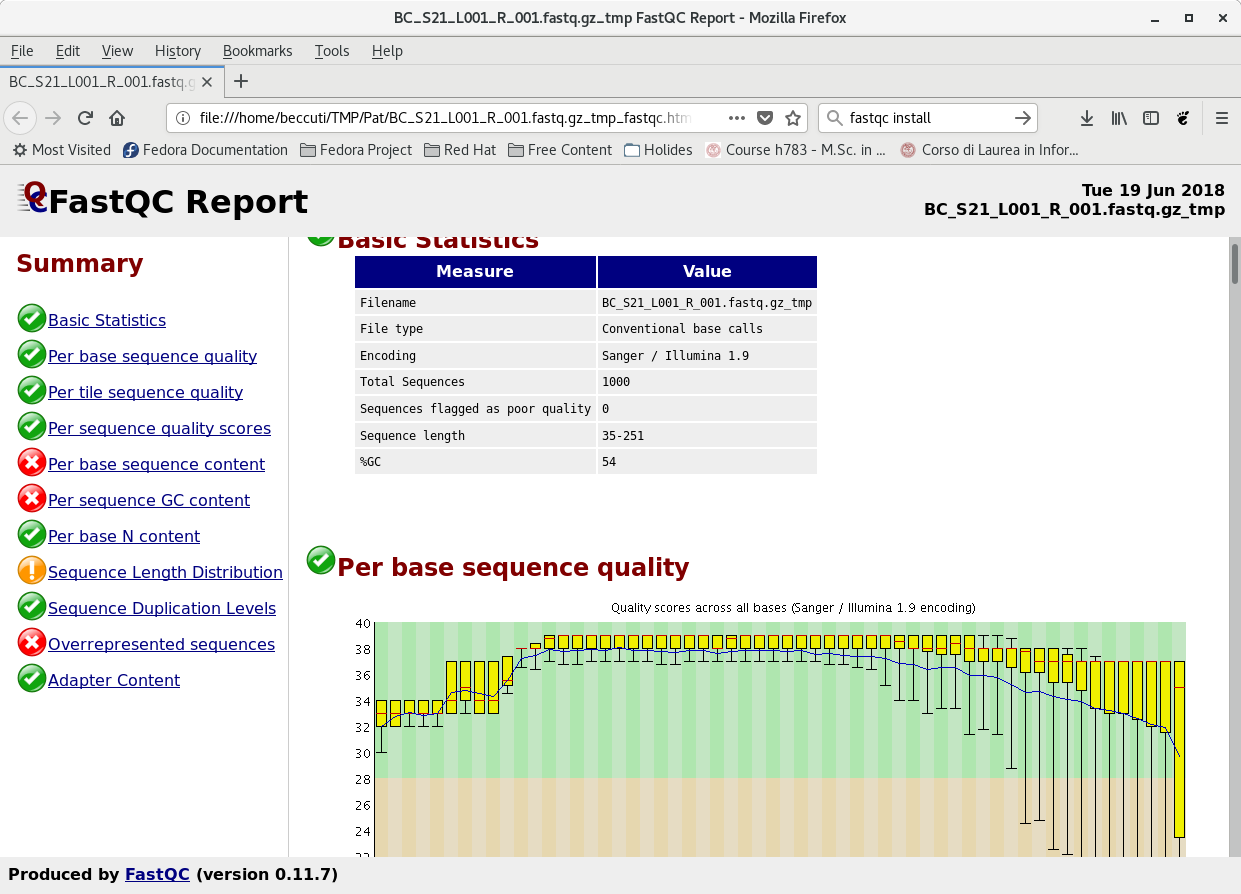
\includegraphics[width=0.78\columnwidth]{./Figure/fastqcHTML}
  			\end{center}	
  						
 \end{itemize}
}


   \frame{
  \frametitle {}
  \vspace{1.5cm}
  \centerline{\Huge \color{NavyBlue} \textbf{\emph{Create a docker image for }}}\vspace{0.05cm}
  \centerline{\Huge \color{NavyBlue} \textbf{\emph{FastQC tool using dockerfile}}}
  \vspace{0.4cm}
     	\begin{center}
  			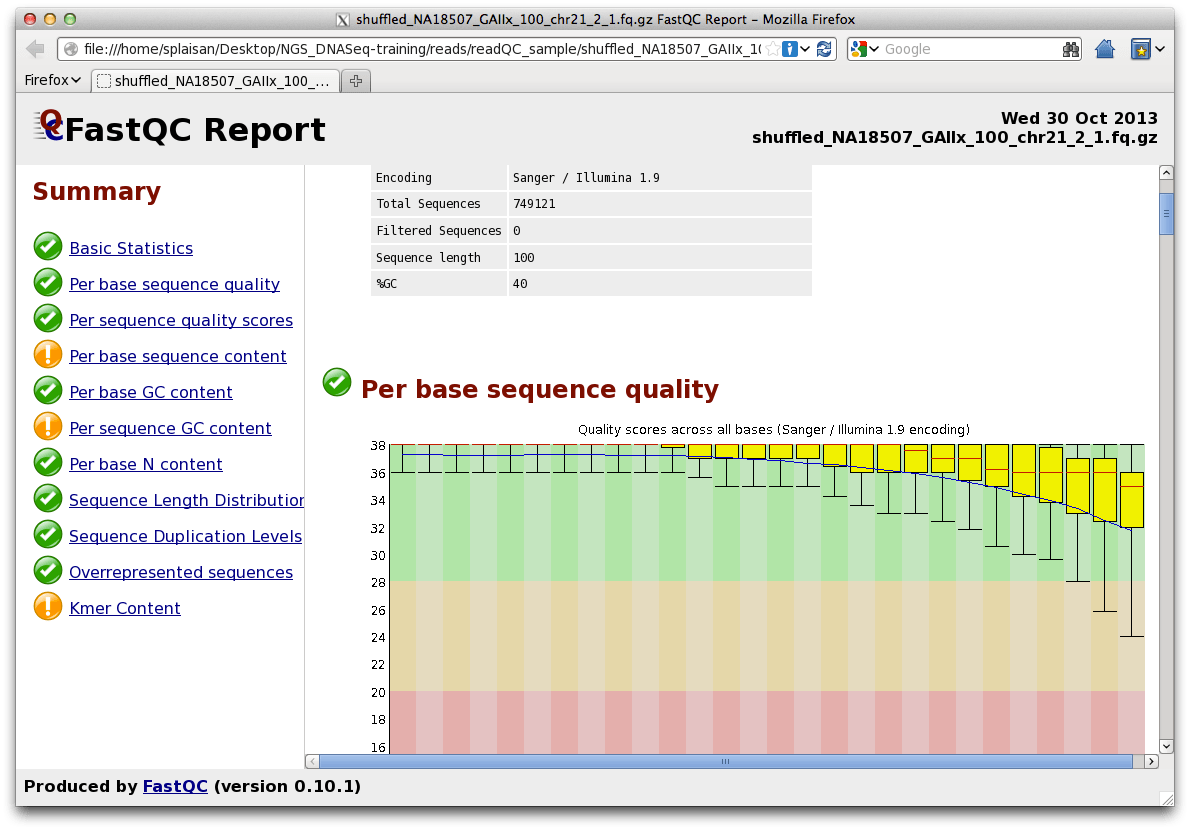
\includegraphics[width=0.60\columnwidth]{./Figure/FastQC}
  		\end{center} 

}


          \frame{
  \frametitle {Create a dockerfile}
  We use \textbf{\color{NavyBlue}gedit} to create our dockerfile; \vspace{0.2cm}
 \begin{center}
  			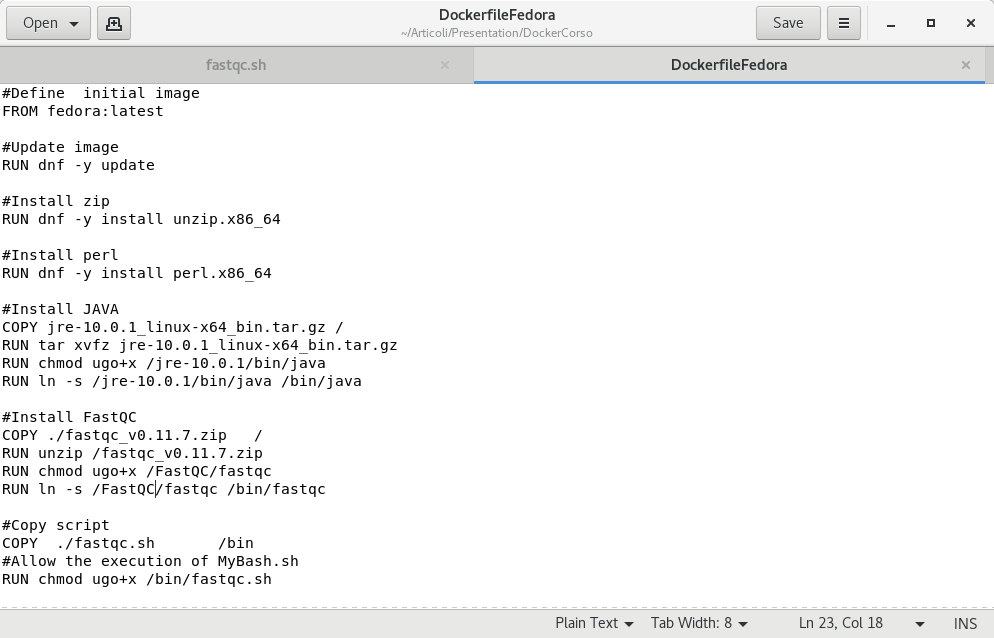
\includegraphics[width=0.95\columnwidth]{./Figure/gedit2}
 \end{center} 
  }

 \frame{
  \frametitle {Create FastQC image with dockerfile}
  
 \emph{\color{PineGreen} docker build -t  ``beccuti/fastqc2'' . -f DockerfileFedora} can be used to build an image from a Dockerfile.
     	\begin{center}
  			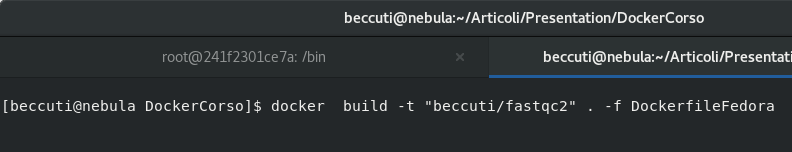
\includegraphics[width=1.00\columnwidth]{./Figure/build2}
  		\end{center}  
  		     	\begin{center}
  			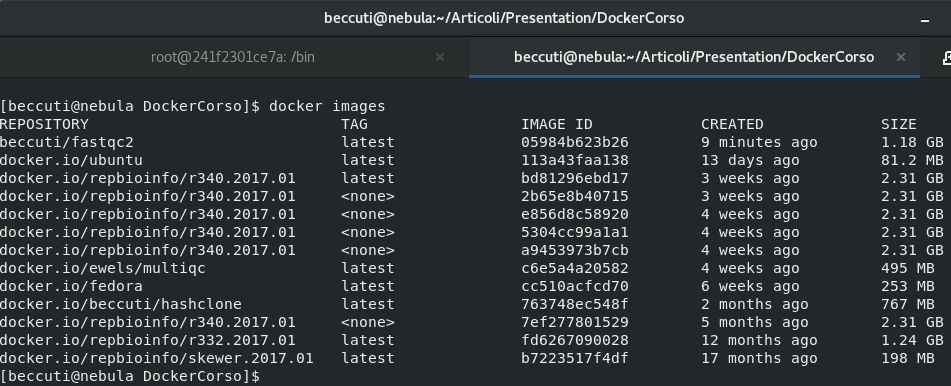
\includegraphics[width=1.00\columnwidth]{./Figure/build3}
  		\end{center}  
  
 } 	
  	

   \frame{
  \frametitle {}
  \vspace{1.5cm}
  \centerline{\Huge \color{NavyBlue} \textbf{\emph{A web server using docker}}}
  \vspace{0.4cm}
     	\begin{center}
  			
\includegraphics[width=0.50\columnwidth]{./Figure/nginxDocker}
  		\end{center} 

}  

\frame{
\frametitle {}
\vspace{1.5cm}
\centerline{\Huge \color{NavyBlue} \textbf{\emph{Networking}}}
\vspace{0.4cm}
\begin{center}
  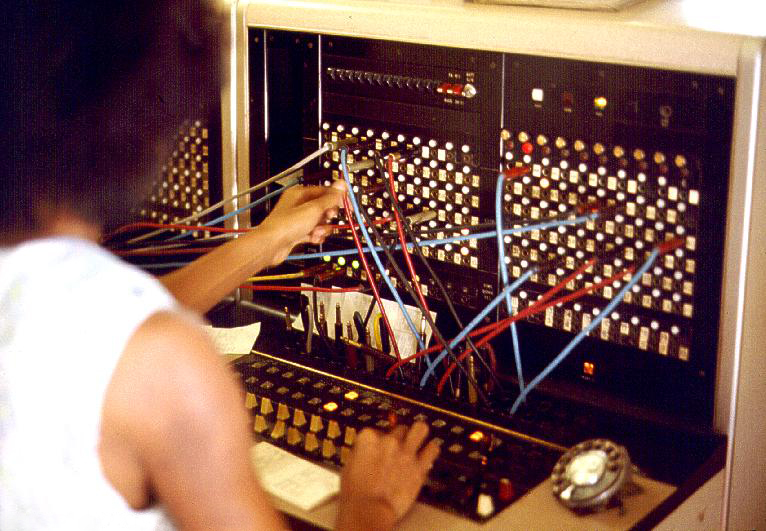
\includegraphics[width=0.60\columnwidth]{./Figure/network/Jersey_Telecom_switchboard_and_operator}
\end{center} 
}


\begin{frame}
\frametitle{Networking}
\begin{itemize}
\item Networking is about communication
\item Text is the simplest way to communicate
\item Protocols are standards for reading and writing text
\end{itemize}
\tiny
\href{https://betterexplained.com/articles/a-simple-introduction-to-computer-networking/}{Ref.}
\normalsize
\end{frame}


\begin{frame}
\frametitle{Networking}
To communicate we must identify the players.\\

Someone's phone number or the address.
\begin{center}
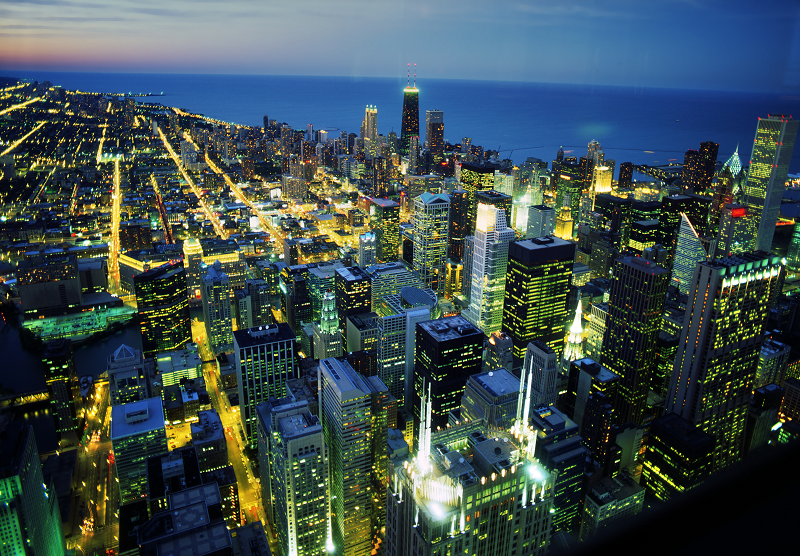
\includegraphics[width=\columnwidth]{./Figure/network/ChicagovanafSearsTower}
\end{center}
\end{frame}


\begin{frame}
\frametitle{Networking}
To communicate we must identify the players.\\

Now the internal door number
\begin{center}
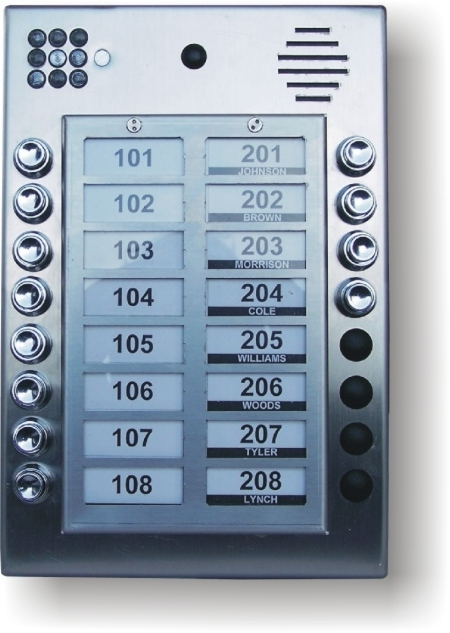
\includegraphics[width=4cm]{./Figure/network/BellGuard_Front_small}
\end{center}
\end{frame}


\begin{frame}
\frametitle{Networking}
To communicate we must identify the players.\\

\begin{columns}
\begin{column}{0.5\textwidth}
\begin{center}
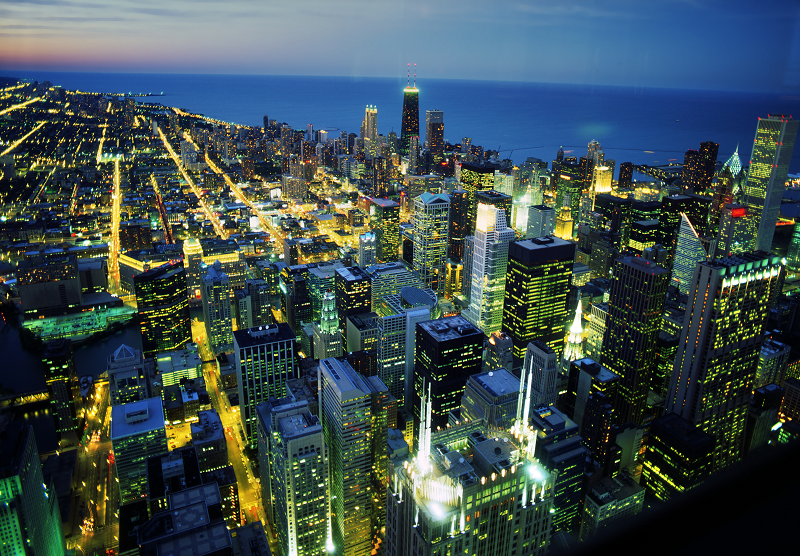
\includegraphics[width=4cm]{./Figure/network/ChicagovanafSearsTower}\\
IP
\end{center}
\end{column}
\begin{column}{0.5\textwidth}
\begin{center}
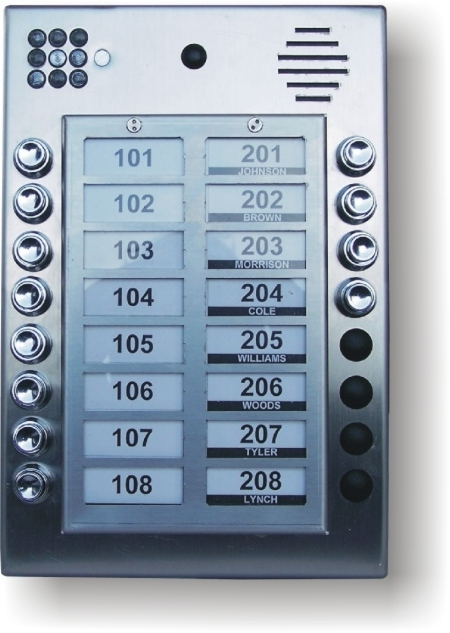
\includegraphics[width=4cm]{./Figure/network/BellGuard_Front_small}\\
PORT
\end{center}
\end{column}
\end{columns}
\end{frame}

\begin{frame}[fragile]
\frametitle{Networking}
A computer is identified by an \textit{IP} number:
\begin{lstlisting}
127.0.0.1

10.0.2.5

172.29.10.1

192.168.1.1
\end{lstlisting}
\end{frame}

\begin{frame}[fragile]
\frametitle{Networking}
IPs can span multiple rangers
\begin{lstlisting}
10.0.0.0 - 10.255.255.255

172.16.0.0 - 172.31.255.255

192.168.0.0 - 192.168.255.255
\end{lstlisting}
\end{frame}

\begin{frame}
\frametitle{Networking}
Usually an IP corresponds to a single network card.
\end{frame}

\begin{frame}
\frametitle{Networking}
WiFi is a radio network card so has an IP.
\end{frame}




\begin{frame}
\frametitle{Networking}
\begin{itemize}
\item Networking is about communication
\item Text is the simplest way to communicate
\item Protocols are standards for reading and writing text
\item Ports are channels from which communications pass-thought
\end{itemize}
\tiny
\href{https://betterexplained.com/articles/a-simple-introduction-to-computer-networking/}{Ref.}
\normalsize
\end{frame}



   \frame{
  \frametitle {A web server using docker}
	This requires the following tasks:\vspace{0.4cm}
	\begin{itemize}
	\item Download \textbf{\color{NavyBlue} nginx} docker image;\vspace{0.2cm}
	\item Execute this image using  the option \emph{\color{PineGreen}-p 80:80} to inform Docker that we want to expose the port 80. 
	\end{itemize}	  
  
    }
    
\frame{
\frametitle{A web server using docker}
    	\begin{center}
  			
\includegraphics[width=0.50\columnwidth]{./Figure/nginx}
  		\end{center} 

\begin{itemize}
\item It is a HTTP server software with focus on core web server and proxy features;\vspace{0.2cm}
\item It was developed to provide   high concurrency, high performance and low memory usage;\vspace{0.2cm}
\item It is able to scale incredibly far with limited resources.
\end{itemize}
}  
   \frame{
  \frametitle {Download nginx docker image}
  \begin{itemize}
  	\item Download nginx image;   	 
  	\end{itemize}
  	          	\begin{center}
  			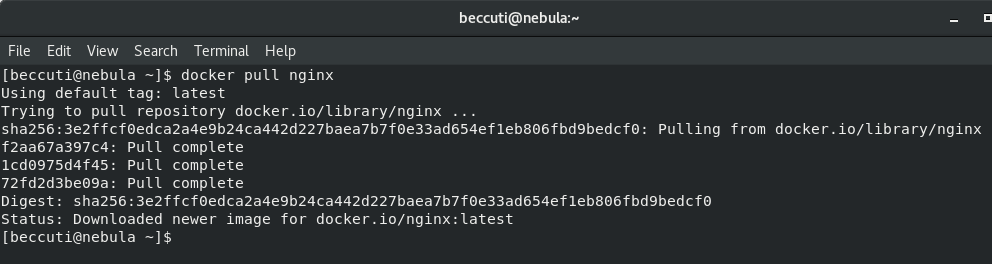
\includegraphics[width=1.0\columnwidth]{./Figure/pullnginx}
  		\end{center}	
  		
	
  		} 
   
 	     \frame{
\frametitle{Execute nginx docker image} 
  
 \emph{\color{PineGreen} docker run -p 80:80 nginx} must be used to star our web server on port 80.
     	\begin{center}
  			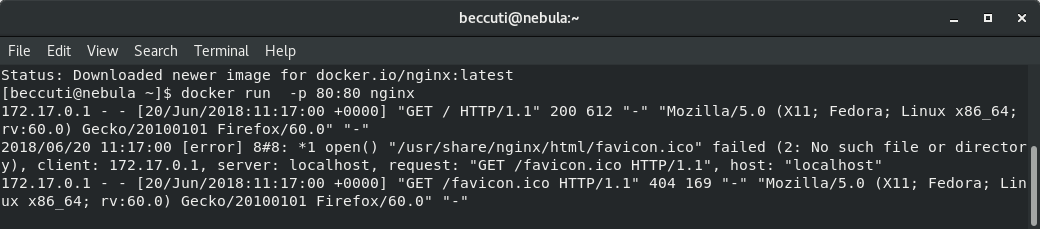
\includegraphics[width=1.00\columnwidth]{./Figure/runnginx}
  		\end{center}  
  	\begin{center}
  			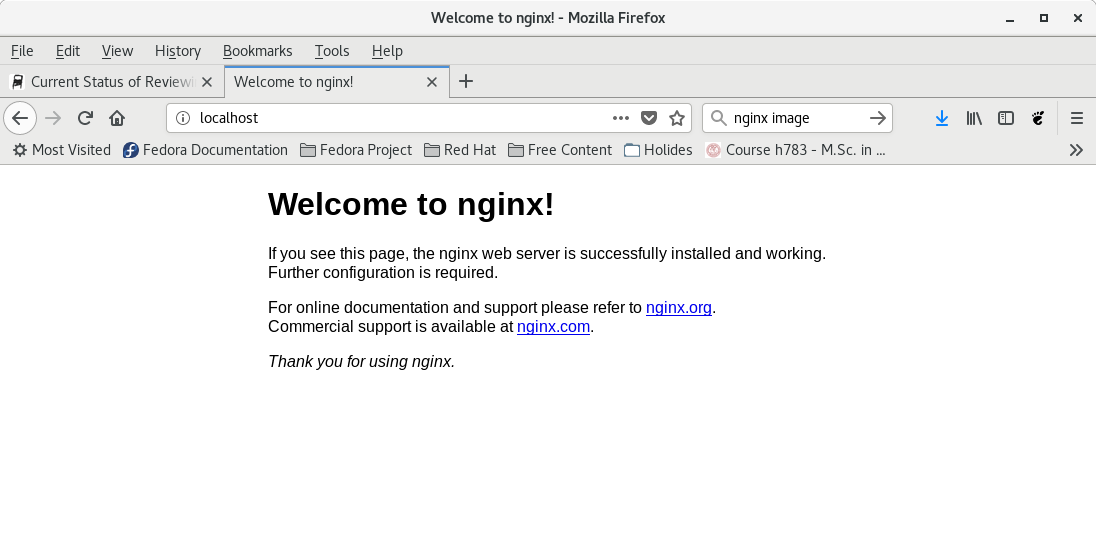
\includegraphics[width=0.95\columnwidth]{./Figure/webnginx}
  		\end{center} 
 }  	
 
   \frame{
\frametitle{Execute nginx docker image}

\textbf{\color{NavyBlue}How to use nginx to visualize fastqc output:}
\vspace{0.4cm}
\begin{itemize}
\item Update nginx image with \textbf{\color{NavyBlue}vi} command;\vspace{0.2cm}
\item Modify   \textbf{\color{NavyBlue}/etc/nginx/conf.d/default.conf}  adding     \emph{\color{PineGreen}autoindex on;} in  \textbf{\color{NavyBlue}location /} block;\vspace{0.2cm}
\item Execute nginx mounting the folder containing fastqc output in \textbf{\color{NavyBlue}/local/shared/nginx/html}.
\end{itemize}  

    	\begin{center}
  			
\includegraphics[width=0.50\columnwidth]{./Figure/nginx} \hspace{0.5cm} 
  			
\includegraphics[width=0.15\columnwidth]{./Figure/QC}
  		\end{center} 
  		    
  	   }  
  
  
   \frame{
\frametitle{Execute nginx docker image} 	   
 \textbf{\color{NavyBlue}How to use nginx to visualize fastqc output:}
\vspace{0.4cm}
\begin{itemize}
\item Update nginx image with \textbf{\color{NavyBlue}vi} command;\vspace{0.2cm}
 \end{itemize} 	   
  	     	\begin{center}
  			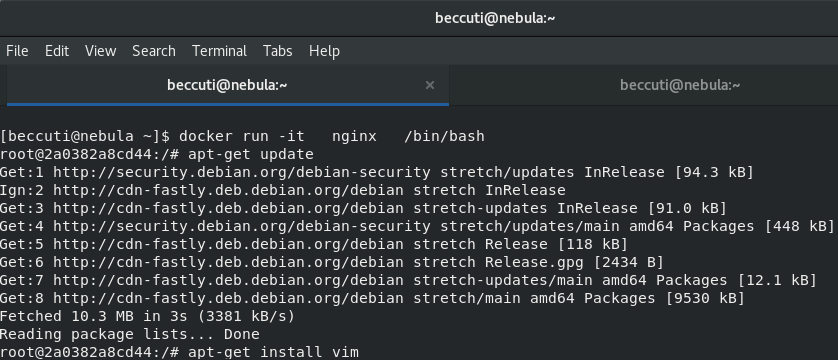
\includegraphics[width=1.0\columnwidth]{./Figure/vimnginx}
  		\end{center}  
  		}
  
    \frame{
\frametitle{Execute nginx docker image} 	   
 \textbf{\color{NavyBlue}How to use nginx to visualize fastqc output:}
\vspace{0.4cm}
\begin{itemize}
\item Modify   \textbf{\color{NavyBlue}/etc/nginx/conf.d/default.conf}  adding     \emph{\color{PineGreen}autoindex on;} in  \textbf{\color{NavyBlue}location /} block;\vspace{0.2cm}
 \end{itemize} 	   
  	     	\begin{center}
  			\includegraphics[width=0.90\columnwidth]{./Figure/confnginx}
  		\end{center}  
  		} 
  		
      \frame{
\frametitle{Execute nginx docker image} 	   
 \textbf{\color{NavyBlue}How to use nginx to visualize fastqc output:}
\vspace{0.4cm}
\begin{itemize}
\item Commit the updates in the images;
 \end{itemize} 	   
  	     	\begin{center}
  			\includegraphics[width=0.90\columnwidth]{./Figure/commitnginx}
  		\end{center}  
  		} 
  		
  			
   		
      \frame{
\frametitle{Execute nginx docker image} 	   
 \textbf{\color{NavyBlue}How to use nginx to visualize fastqc output:}
\vspace{0.4cm}
\begin{itemize}
\item Run the new image \vspace{0.2cm}
\end{itemize}
  	     	\begin{center}
  			\includegraphics[width=1.0\columnwidth]{./Figure/run1ginx}
  		\end{center}
\begin{itemize} 		
\item Option \emph{\color{PineGreen}-v /home/beccuti/TMP/Pat/:/usr/share/nginx/html} is used to set the fastqc output folder as the root directory of web server;\vspace{0.2cm}
\item  Web server is executed in background  using \emph{\color{PineGreen} /usr/sbin/nginx -g "daemon off;"}.
 \end{itemize} 	   
  
  		} 
  		

  			
     \frame{
  \frametitle {}
  \vspace{1.5cm}
  \centerline{\Huge \color{NavyBlue} \textbf{\emph{Deploy services on a cluster }}}
  \centerline{\Huge \color{NavyBlue} \textbf{\emph{using docker swarm}}}
  \vspace{0.4cm}
     	\begin{center}
  			
  			\includegraphics[width=0.40\columnwidth]{./Figure/dockerswarm}
  		\end{center} 

}		 		
  

     \frame{
  \frametitle {Deploy services on a cluster }
  We will use  \emph{\color{NavyBlue} docker-machine} to create two virtual nodes. \vspace{0.4cm}
  \begin{itemize}
  \item It is a tool that lets you install Docker Engine on virtual hosts; \vspace{0.2cm}
  \item It requires an Hypervisor (e.g. Oracle VirtualBox) installed on the machine;\vspace{0.2cm}
  \end{itemize}
  	\begin{center}
  \includegraphics[width=0.30\columnwidth]{./Figure/dockermachine}
  		\end{center} 

}	  	


     \frame{
\frametitle{Deploy services on a cluster } 
  \vspace{0.1cm}
 \emph{\color{PineGreen} docker-machine create -\;-driver virtualbox myvm1} creates and starts a VirtualBox VM with Docker running.
     	\begin{center}
  			\includegraphics[width=1.00\columnwidth]{./Figure/createvm}
  		\end{center}  
 }  	  
  	

     \frame{
\frametitle{Deploy services on a cluster } 
  
 \emph{\color{PineGreen} docker-machine ls} returns the list of the created VirtualBox VMs.  \vspace{0.1cm}
     	\begin{center}
  			\includegraphics[width=0.90\columnwidth]{./Figure/lsvm}
  		\end{center}   
 \emph{\color{PineGreen} docker-machine stop myvm1} stops \textbf{\color{NavyBlue}myvm1} VM.  \vspace{-0.1cm}
     	\begin{center}
  			\includegraphics[width=0.90\columnwidth]{./Figure/stopvm}
  		\end{center} 
}

     \frame{
\frametitle{Deploy services on a cluster } 
    		 \emph{\color{PineGreen} docker-machine start myvm1} starts \textbf{\color{NavyBlue}myvm1} VM.  \vspace{0.3cm}
     	\begin{center}
  			\includegraphics[width=0.90\columnwidth]{./Figure/runvm}
  		\end{center}  
 }  	    	
  
  
   \frame{
\frametitle{Deploy services on a cluster } 
  
 \emph{\color{PineGreen} docker-machine rm myvm1} removes \textbf{\color{NavyBlue}myvm1} VM.  \vspace{0.1cm}
     	\begin{center}
  			\includegraphics[width=0.90\columnwidth]{./Figure/rmvm}
  		\end{center}

 } 
 
    \frame{
\frametitle{Deploy services on a cluster } 
  
   		 \emph{\color{PineGreen} docker-machine ssh myvm1} can be used to access  \textbf{\color{NavyBlue}myvm1} VM.  \vspace{0.2cm}
     	\begin{center}
  			\includegraphics[width=1.0\columnwidth]{./Figure/sshvm}
  		\end{center}    
}
 
   
   \frame{
\frametitle{Deploy services on a cluster } 
   	    	  
   \emph{\color{PineGreen} docker-machine ssh myvm1 "docker ps -a"} can be used to execute commands on \textbf{\color{NavyBlue}myvm1} VM.  \vspace{0.2cm}
     	\begin{center}
  			\includegraphics[width=1.00\columnwidth]{./Figure/execvm}
  		\end{center} 
  		}

   \frame{
\frametitle{Deploy services on a cluster }  
\emph{\color{PineGreen} docker-machine ssh  myvm1 "docker swarm init --advertise-addr 192.168.99.102"}  is used to initialize the swarm and set \textbf{\color{NavyBlue}myvm1} as manager.
     	\begin{center}
  			\includegraphics[width=1.00\columnwidth]{./Figure/initswarm}
  		\end{center} 
\emph{\color{PineGreen} docker-machine ssh  myvm2 "docker swarm join --token SWMTKN-1-430vpzpm8ves6whcy8ox34vlyrrmutinoewrzcaaqix32h917f-7bml90kfo5j1toxmql19hfsmh 192.168.99.102:2377"}  is used to add \textbf{\color{NavyBlue}myvm2} into the  swarm.
     	\begin{center}
  			\includegraphics[width=1.00\columnwidth]{./Figure/addswarm}
  		\end{center} 

}
 
 
    \frame{
\frametitle{}
 \centerline{\Huge \color{NavyBlue} \textbf{\emph{ Deploy services}} }\vspace{0.1cm} \centerline{\Huge \color{NavyBlue} \textbf{\emph{into a Docker swarm}}}
     	\begin{center}
  			
  			\includegraphics[width=0.40\columnwidth]{./Figure/dockerswarm}
  		\end{center} 
} 
  
   \frame{
\frametitle{Deploy services on a cluster } 
   	    	  
   \emph{\color{PineGreen} docker-machine ssh myvm1 "docker node ls"} provides information about the swarm nodes.  \vspace{-0.1cm}
     	\begin{center}
  			\includegraphics[width=1.0\columnwidth]{./Figure/nodelsswarm}
  		\end{center} 		
   \emph{\color{PineGreen}docker-machine ssh  myvm1 "docker node update -\;-availability drain  myvm2"} makes a node inactive.  \vspace{-0.1cm}
     	\begin{center}
  			\includegraphics[width=1.0\columnwidth]{./Figure/nodeinacswarm}
  		\end{center} 
  		}   		
  	
   \frame{
\frametitle{Deploy services on a cluster } 
   	    	
   \emph{\color{PineGreen}docker-machine ssh  myvm1 "docker node update -\;-availability active  myvm2"} makes a node inactive.  \vspace{0.2cm}
     	\begin{center}
  			\includegraphics[width=1.0\columnwidth]{./Figure/nodeactswarm}
  		\end{center} 
  		}   	  	
  		
  	  		
  		
  	   \frame{
\frametitle{Deploy services on a cluster } 
   	    	  
   \emph{\color{PineGreen} docker-machine ssh myvm1 "docker service create   -\;-name my-web   -\;-publish published=80,target=80 -\;-replicas=1     nginx"} starts one service on a node.  \vspace{-0.1cm}
     	\begin{center}
  			\includegraphics[width=1.00\columnwidth]{./Figure/serviceswarm}
  		\end{center} 	
  				
  \emph{\color{PineGreen}docker-machine ssh  myvm1 "docker  service ls"} and \emph{\color{PineGreen}docker-machine ssh  myvm1 "docker service  ps my-web"}
    return information on services.
    
       	\begin{center}
  			\includegraphics[width=1.00\columnwidth]{./Figure/serviceinfoswarm}
  		\end{center}  
  		}	
    		
  	   \frame{
\frametitle{Deploy services on a cluster } 
   	    	  
   \emph{\color{PineGreen}  docker-machine ssh  myvm1 "docker service scale my-web=2" 	} can be used to scale a service.  \vspace{-0.1cm}
     	\begin{center}
  			\includegraphics[width=1.0\columnwidth]{./Figure/scaleswarm}
  		\end{center} 	

       	\begin{center}
  			\includegraphics[width=1.0\columnwidth]{./Figure/serviceinfoswarm2}
  		\end{center}  
  		}		
  		
  	 	   \frame{
\frametitle{Deploy services on a cluster } 
   	    	  
   \emph{\color{PineGreen} docker-machine ssh  myvm1 "docker service create -\;-name my-web   -\;-publish published=80,target=80   - -mode global  nginx"
 	} can be use to automatically allocate a service on all the nodes  \vspace{-0.1cm}
     	\begin{center}
  			\includegraphics[width=1.0\columnwidth]{./Figure/serviceglobalswarm}
  		\end{center} 	

       	\begin{center}
  			\includegraphics[width=1.0\columnwidth]{./Figure/serviceglobalswarm2}
  		\end{center}  
  		}		
	
    		
  	 	   \frame{
\frametitle{Deploy services on a cluster } 
\textbf{\color{NavyBlue}How to execute a one-shot service using swam}\vspace{0.4cm}
\begin{itemize}
\item Our goal is to use fastqc image\footnote{It must be uploaded in Docker hub} in parallel on the two nodes; \vspace{0.2cm}
\item Data can be shared using Virtualbox shared folder (i.e. \textbf{\color{NavyBlue}/hosthome}); \vspace{0.2cm}
\item We create two folders with containing fastq files. (i.e. \textbf{\color{NavyBlue}d1/} and \textbf{\color{NavyBlue}d2/});\vspace{0.2cm}
\item Option  \emph{\color{PineGreen} -\;-restart-condition=``none" } can be used for running  one-shot service;\vspace{0.2cm}
\item Option  \emph{\color{PineGreen} --mount type=bind,src=$\langle SOURCE \rangle$ ,dst= $\langle DESTINATION \rangle$} can be used for mounting the input data folder;
\end{itemize}

}		

  	 	   \frame{
\frametitle{Deploy services on a cluster } 
\textbf{\color{NavyBlue}How to execute a one-shot service using swam}\\\vspace{0.4cm}
\emph{\color{PineGreen}docker-machine  ssh   myvm1\\
\hspace{0.5cm}"docker service create -\;-replicas 1 -\;-name S1 -\;-user 1000  \\
\hspace{0.5cm}-\;-restart-condition="none"   \\
\hspace{0.5cm}-\;-mount type=bind,\\
\hspace{0.5cm}src=/hosthome/beccuti/Articoli/Presentation/DockerCorso/data/d2,\\
\hspace{0.5cm}dst=/data/scratch \\
\hspace{0.5cm}docker.io/beccuti/fastqc2   /bin/fastqc.sh"}

       	\begin{center}
  			\includegraphics[width=1.0\columnwidth]{./Figure/serviceoneswarm}
  		\end{center} 

} 


 	 	   \frame{
\frametitle{Deploy services on a cluster } 
\textbf{\color{NavyBlue}How to execute a one-shot service using swam}\\\vspace{0.4cm}
\emph{\color{PineGreen}docker-machine  ssh   myvm1\\
\hspace{0.5cm}"docker service create -\;-replicas 1 -\;-name S2 -\;-user 1000  \\
\hspace{0.5cm}-\;-restart-condition="none"   \\
\hspace{0.5cm}-\;-mount type=bind,\\
\hspace{0.5cm}src=/hosthome/beccuti/Articoli/Presentation/DockerCorso/data/d1,\\
\hspace{0.5cm}dst=/data/scratch \\
\hspace{0.5cm}docker.io/beccuti/fastqc2   /bin/fastqc.sh"}

       	\begin{center}
  			\includegraphics[width=1.0\columnwidth]{./Figure/serviceoneswarm1}
  		\end{center} 

} 


  	 	   \frame{
\frametitle{Deploy services on a cluster } 
\textbf{\color{NavyBlue}How to execute a one-shot service using swam}\vspace{0.4cm}
       	\begin{center}
  			\includegraphics[width=1.0\columnwidth]{./Figure/serviceoneps}
  		\end{center} 
  		       	\begin{center}
  			\includegraphics[width=1.0\columnwidth]{./Figure/serviceoneps1}
  		\end{center} 
}
 		

  		\frame{
\frametitle{Conclusion}
In this training day:\vspace{0.1cm}
\begin{enumerate}
\item A short introduction  recalling the concepts described in the first day\vspace{0.1cm}
\begin{itemize}
\item Virtualization: Virtual Machines and containers; \vspace{0.1cm}
\item Containers in Linux: Docker project; \vspace{0.1cm}
\end{itemize}

\item A simple example: how to embed an application  in docker image; \vspace{0.1cm}
\item Create a docker image for FastQC tool;\vspace{0.1cm}
\item A web server  using docker;\vspace{0.1cm}
\item Deploy services on a cluster using docker swarm.
\end{enumerate}
\centerline{\includegraphics[scale=0.22]{./Figure/end}}
}
 		
 	
\frame{
\frametitle{}
\vspace{2.0cm}
\centerline{\includegraphics[scale=0.55]{./Figure/thanks.jpg}}
}


\frame{
\frametitle {}
\vspace{2cm}
\centerline{\Huge \color{NavyBlue} \textbf{\emph{Storage}}}
\vspace{0.5cm}
}
\frame{
\frametitle{Docker Storage}
Every piece of data in Docker is a layer.
\vspace{0.4cm}
Layers can be (are) resued when possible.
\vspace{0.4cm}
\includegraphics[width=0.50\columnwidth]{./Figure/docker-064-046}
}

\frame{
\frametitle{Docker Storage}
\framesubtitle{Layers}
Layers are a sort of snapshots of a filesystem
\vspace{0.4cm}
Usually are in readonly mode
\vspace{0.4cm}
To every new container a \it{Thin} r/w layer is created. In this layer the container can store its own data.
}

\begin{frame}[fragile]
\frametitle{Docker Storage}
\framesubtitle{Layers}
\begin{columns}
\begin{column}{.65\textwidth}
\begin{lstlisting}
FROM ubuntu:15.04
COPY ./app
RUN make /app
CMD python /app/app.py
\end{lstlisting}
\end{column}
\begin{column}{.35\textwidth}
\includegraphics[width=1\columnwidth]{./Figure/docker-064-046}
\end{column}
\end{columns}
\end{frame}

\begin{frame}[fragile]
\frametitle{Docker Storage}
\framesubtitle{Pull and Storage}
\begin{lstlisting}
$ docker pull ubuntu:15.04

15.04: Pulling from library/ubuntu
1ba8ac955b97: Pull complete
f157c4e5ede7: Pull complete
0b7e98f84c4c: Pull complete
a3ed95caeb02: Pull complete
Digest: sha256:5e279a9df07990286cce22e1b0f5b049062
	9ca6d187698746ae5e28e604a640e
Status: Downloaded newer image for ubuntu:15.04
\end{lstlisting}
\end{frame}

\begin{frame}[fragile]
\frametitle{Docker Storage}
\framesubtitle{Pull and Storage}
\begin{lstlisting}
$ docker pull ubuntu:18.04
18.04: Pulling from library/ubuntu
124c757242f8: Pull complete
9d866f8bde2a: Pull complete
fa3f2f277e67: Pull complete
398d32b153e8: Pull complete
afde35469481: Pull complete
Digest: sha256:de774a3145f7ca4f0bd144c7d4ffb2931e0
	6634f11529653b23eba85aef8e378
Status: Downloaded newer image for ubuntu:18.04
\end{lstlisting}
\end{frame}


\begin{frame}[fragile]
\frametitle{Docker Storage}
\framesubtitle{Pull and Storage}
\begin{lstlisting}
$ docker images -f reference='ubuntu'

REPOSITORY   TAG     IMAGE ID      CREATED      SIZE
ubuntu       18.04   cd6d8154f1e1  2 weeks ago  84.1MB
ubuntu       16.04   2dc7f0e4fc33  2 years ago  122MB
ubuntu       14.04   54060fb55e83  3 years ago  188MB
\end{lstlisting}
\end{frame}

\begin{frame}[fragile]
\frametitle{Docker Storage}
\framesubtitle{Pull and Storage}
\begin{lstlisting}
$ sudo find /var/lib/docker -name cd6d81*

/var/lib/docker/image/aufs/imagedb/content/sha256/
	cd6d8154f1e16e38493c3c2798977c5e142be5e5d41403
	ca89883840c6d51762

\end{lstlisting}
\end{frame}

\begin{frame}
\frametitle{Docker Storage}
\framesubtitle{Drivers}
\includegraphics[width=1.0\columnwidth]{./Figure/docker-070-052}
\end{frame}

\begin{frame}
\frametitle{Docker Storage}
\framesubtitle{Drivers}
\begin{itemize}
\item aufs, overlay, overlay2: work at file level, memory efficient but layers can grow and become inefficient with high I/O
\item devicemapper,btrfs, zfs: block-level storage, works with write-heavy I/O
\item btrfs, zfs: require a lot of memory
\item zfs: is a good choice for high-density workloads such as PaaS
\item overlay: works better with many layers and small files compared to overlay2
\end{itemize}
\end{frame}


\begin{frame}
\frametitle{Docker Storage}
\framesubtitle{Drivers}

How to choose the driver:
\begin{itemize}
\item Perform tests based on your hardware with your sysadmin
\item Check the stability of the driver and decide your stability policy
\item If you have an expertise in house use it
\item Some drivers works best on some Linux distro
\item Perform tests on real workloads
\end{itemize}
\end{frame}

\begin{frame}
\frametitle{Docker Storage}
\framesubtitle{Drivers}
\it{!!! WARING !!!}
\vspace{0.4cm}
You can not mix drivers
\vspace{0.4cm}
Each driver has its set of images and containers
\vspace{0.4cm}
Migration is not possible
\end{frame}


\begin{frame}
\frametitle{Docker Storage}
\framesubtitle{Layers}
Layers are a sort of snapshots of a filesystem
\vspace{0.4cm}
Usually are in readonly mode
\vspace{0.4cm}
To every new container a \it{Thin} r/w layer is created. In this layer the container can store its own data.
\end{frame}

\begin{frame}
\frametitle{Docker Storage}
\framesubtitle{Thin layers}
\includegraphics[width=0.5\columnwidth]{./Figure/docker-065-047}
\end{frame}


\begin{frame}
\frametitle{Docker Storage}
\framesubtitle{Thin layers and Data}
A writable container layer is created every time a container starts and it is where data are stored.
\vspace{0.4cm}
When a container is not running:
\begin{itemize}
\item Data does not persist
\item Sharing data with other container is very very ... very complicated
\item Your host machine own the writable layer, moving the layer is not that simple
\item Not the best option for high I/O, layers can be asynchronous 
\end{itemize}
\end{frame}

\begin{frame}[fragile]
\frametitle{Docker Storage}
\framesubtitle{Thin layers}
\begin{lstlisting}
$ docker run -dit --name my_container_1
           acme/my-final-image:1.0 bash

c36785c423ec7e0422b2af7364a7ba4da6146cbba7981a0951
	fcc3fa0430c409


$ docker run -dit --name my_container_2 
           acme/my-final-image:1.0 bash
		   
dcad7101795e4206e637d9358a818e5c32e13b349e62b00bf0
	5cd5a4343ea513

...
\end{lstlisting}
\end{frame}

\begin{frame}[fragile]
\frametitle{Docker Storage}
\framesubtitle{Thin layers, where are }
\begin{lstlisting}
$ sudo du -shL /var/lib/docker/containers/*
32K /var/lib/docker/containers/1a174fc216cccf18ec7
	d4fe14e008e30130b11ede0f0f94a87982e310cf2e765
32K /var/lib/docker/containers/1e7264576d78a3134fb
	af7829bc24b1d96017cf2bc046b7cd8b08b5775c33d0c
32K /var/lib/docker/containers/38fa94212a419a082e6
	a6b87a8e2ec4a44dd327d7069b85892a707e3fc818544
32K /var/lib/docker/containers/c36785c423ec7e0422b
	2af7364a7ba4da6146cbba7981a0951fcc3fa0430c409
32K /var/lib/docker/containers/dcad7101795e4206e63
	7d9358a818e5c32e13b349e62b00bf05cd5a4343ea513 
\end{lstlisting}
\end{frame}

\begin{frame}[fragile]
\frametitle{Docker Storage}
\framesubtitle{Container and Size}
Running a plain Ubuntu 18.04
\vspace{0.4cm}
\begin{lstlisting}
$ docker run ubuntu -it ubuntu:18.04 bash
\end{lstlisting}
\vspace{0.4cm}
\it{Note} detach from the container using \lstinline!Ctrl-P! + \lstinline!Ctrl-Q!
\end{frame}

\begin{frame}[fragile]
\frametitle{Docker Storage}
\framesubtitle{Container and Size}
\begin{lstlisting}
$ docker ps -s


| CONTAINER ID | IMAGE        | SIZE                |

| 0e7438744a0a | ubuntu:18.04 | 0B (virtual 84.1MB) |
\end{lstlisting}
\end{frame}

\begin{frame}[fragile]
\frametitle{Docker Storage}
\framesubtitle{Container and Size}
Updating the \lstinline!apt! database
\vspace{0.4cm}
\begin{lstlisting}
$ docker attach 0e74

$ apt update


| CONTAINER ID | IMAGE        | SIZE                   |

| 0e7438744a0a | ubuntu:18.04 | 41.7MB (virtual 126MB) |
\end{lstlisting}
\end{frame}

\begin{frame}[fragile]
\frametitle{Docker Storage}
\framesubtitle{Container and Size}
Upgrading the \lstinline!apt! database
\vspace{0.4cm}
\begin{lstlisting}
$ apt upgrade


| CONTAINER ID | IMAGE        | SIZE                   |

| 0e7438744a0a | ubuntu:18.04 | 42.6MB (virtual 127MB) |
\end{lstlisting}
\end{frame}

\begin{frame}[fragile]
\frametitle{Docker Storage}
\framesubtitle{Container and Size}
Installing \lstinline!wget!
\vspace{0.4cm}
\begin{lstlisting}
$ apt install wget


| CONTAINER ID | IMAGE        | SIZE                   |

| 0e7438744a0a | ubuntu:18.04 | 49.1MB (virtual 133MB) |
\end{lstlisting}
\end{frame}





\frame{
\frametitle {}
\vspace{2cm}
\centerline{\Huge \color{NavyBlue} \textbf{\emph{Swarm}}}
\vspace{0.5cm}
}
\begin{frame}
\frametitle{Swarm}
\framesubtitle{Overview}
Multiple Docker hosts can be managed in a centralized manner using an inner feature of Docker: \textbf{\textit{Swarm}}
\end{frame}

\begin{frame}
\frametitle{Swarm}
\framesubtitle{Overview}
\begin{itemize}
\item Cluster management
\item Decentralized design (one is all)
\item Declarative service model
\item Scaling
\item Desired state reconciliation
\item Multi-host networking
\item Service discovery
\item Load balancing
\item Secure by default (TLS)
\item Rolling updates
\end{itemize}
\end{frame}

\begin{frame}
\frametitle{Swarm}
\framesubtitle{Overview}
A generic Docker Host is a \textit{Node} in the Swarm.
\end{frame}

\begin{frame}
\frametitle{Swarm}
\framesubtitle{Overview}
A generic Docker Host is a \textit{Node} in the Swarm.
\vspace{0.4}
A Node can be:
\begin{itemize}
\item Manger: dispatches task to workers; orchestrate and manage the cluster
\item Worker: executes a task  
\end{itemize}
\end{frame}

\frame{
\frametitle {}
\vspace{2cm}
\centerline{\Huge \color{NavyBlue} \textbf{\emph{Swarm}}}
\vspace{0.5cm}
}

     \frame{
  \frametitle {Deploy services on a cluster }
  We will use  \emph{\color{NavyBlue} docker-machine} to create two virtual nodes. \vspace{0.4cm}
  \begin{itemize}
  \item It is a tool that lets you install Docker Engine on virtual hosts; \vspace{0.2cm}
  \item It requires an Hypervisor (e.g. Oracle VirtualBox) installed on the machine;\vspace{0.2cm}
  \end{itemize}
  	\begin{center}
  \includegraphics[width=0.30\columnwidth]{./Figure/dockermachine}
  		\end{center} 

}	  	


     \frame{
\frametitle{Deploy services on a cluster } 
  \vspace{0.1cm}
 \emph{\color{PineGreen} docker-machine create -\;-driver virtualbox myvm1} creates and starts a VirtualBox VM with Docker running.
     	\begin{center}
  			\includegraphics[width=1.00\columnwidth]{./Figure/createvm}
  		\end{center}  
 }  	  
  	

     \frame{
\frametitle{Deploy services on a cluster } 
  
 \emph{\color{PineGreen} docker-machine ls} returns the list of the created VirtualBox VMs.  \vspace{0.1cm}
     	\begin{center}
  			\includegraphics[width=0.90\columnwidth]{./Figure/lsvm}
  		\end{center}   
 \emph{\color{PineGreen} docker-machine stop myvm1} stops \textbf{\color{NavyBlue}myvm1} VM.  \vspace{-0.1cm}
     	\begin{center}
  			\includegraphics[width=0.90\columnwidth]{./Figure/stopvm}
  		\end{center} 
}

     \frame{
\frametitle{Deploy services on a cluster } 
    		 \emph{\color{PineGreen} docker-machine start myvm1} starts \textbf{\color{NavyBlue}myvm1} VM.  \vspace{0.3cm}
     	\begin{center}
  			\includegraphics[width=0.90\columnwidth]{./Figure/runvm}
  		\end{center}  
 }  	    	
  
  
   \frame{
\frametitle{Deploy services on a cluster } 
  
 \emph{\color{PineGreen} docker-machine rm myvm1} removes \textbf{\color{NavyBlue}myvm1} VM.  \vspace{0.1cm}
     	\begin{center}
  			\includegraphics[width=0.90\columnwidth]{./Figure/rmvm}
  		\end{center}

 } 
 
    \frame{
\frametitle{Deploy services on a cluster } 
  
   		 \emph{\color{PineGreen} docker-machine ssh myvm1} can be used to access  \textbf{\color{NavyBlue}myvm1} VM.  \vspace{0.2cm}
     	\begin{center}
  			\includegraphics[width=1.0\columnwidth]{./Figure/sshvm}
  		\end{center}    
}
 
   
   \frame{
\frametitle{Deploy services on a cluster } 
   	    	  
   \emph{\color{PineGreen} docker-machine ssh myvm1 "docker ps -a"} can be used to execute commands on \textbf{\color{NavyBlue}myvm1} VM.  \vspace{0.2cm}
     	\begin{center}
  			\includegraphics[width=1.00\columnwidth]{./Figure/execvm}
  		\end{center} 
  		}

   \frame{
\frametitle{Deploy services on a cluster }  
\emph{\color{PineGreen} docker-machine ssh  myvm1 "docker swarm init --advertise-addr 192.168.99.102"}  is used to initialize the swarm and set \textbf{\color{NavyBlue}myvm1} as manager.
     	\begin{center}
  			\includegraphics[width=1.00\columnwidth]{./Figure/initswarm}
  		\end{center} 
\emph{\color{PineGreen} docker-machine ssh  myvm2 "docker swarm join --token SWMTKN-1-430vpzpm8ves6whcy8ox34vlyrrmutinoewrzcaaqix32h917f-7bml90kfo5j1toxmql19hfsmh 192.168.99.102:2377"}  is used to add \textbf{\color{NavyBlue}myvm2} into the  swarm.
     	\begin{center}
  			\includegraphics[width=1.00\columnwidth]{./Figure/addswarm}
  		\end{center} 

}
 
 
    \frame{
\frametitle{}
 \centerline{\Huge \color{NavyBlue} \textbf{\emph{ Deploy services}} }\vspace{0.1cm} \centerline{\Huge \color{NavyBlue} \textbf{\emph{into a Docker swarm}}}
     	\begin{center}
  			
  			\includegraphics[width=0.40\columnwidth]{./Figure/dockerswarm}
  		\end{center} 
} 
  
   \frame{
\frametitle{Deploy services on a cluster } 
   	    	  
   \emph{\color{PineGreen} docker-machine ssh myvm1 "docker node ls"} provides information about the swarm nodes.  \vspace{-0.1cm}
     	\begin{center}
  			\includegraphics[width=1.0\columnwidth]{./Figure/nodelsswarm}
  		\end{center} 		
   \emph{\color{PineGreen}docker-machine ssh  myvm1 "docker node update -\;-availability drain  myvm2"} makes a node inactive.  \vspace{-0.1cm}
     	\begin{center}
  			\includegraphics[width=1.0\columnwidth]{./Figure/nodeinacswarm}
  		\end{center} 
  		}   		
  	
   \frame{
\frametitle{Deploy services on a cluster } 
   	    	
   \emph{\color{PineGreen}docker-machine ssh  myvm1 "docker node update -\;-availability active  myvm2"} makes a node inactive.  \vspace{0.2cm}
     	\begin{center}
  			\includegraphics[width=1.0\columnwidth]{./Figure/nodeactswarm}
  		\end{center} 
  		}   	  	
  		
  	  		
  		
  	   \frame{
\frametitle{Deploy services on a cluster } 
   	    	  
   \emph{\color{PineGreen} docker-machine ssh myvm1 "docker service create   -\;-name my-web   -\;-publish published=80,target=80 -\;-replicas=1     nginx"} starts one service on a node.  \vspace{-0.1cm}
     	\begin{center}
  			\includegraphics[width=1.00\columnwidth]{./Figure/serviceswarm}
  		\end{center} 	
  				
  \emph{\color{PineGreen}docker-machine ssh  myvm1 "docker  service ls"} and \emph{\color{PineGreen}docker-machine ssh  myvm1 "docker service  ps my-web"}
    return information on services.
    
       	\begin{center}
  			\includegraphics[width=1.00\columnwidth]{./Figure/serviceinfoswarm}
  		\end{center}  
  		}	
    		
  	   \frame{
\frametitle{Deploy services on a cluster } 
   	    	  
   \emph{\color{PineGreen}  docker-machine ssh  myvm1 "docker service scale my-web=2" 	} can be used to scale a service.  \vspace{-0.1cm}
     	\begin{center}
  			\includegraphics[width=1.0\columnwidth]{./Figure/scaleswarm}
  		\end{center} 	

       	\begin{center}
  			\includegraphics[width=1.0\columnwidth]{./Figure/serviceinfoswarm2}
  		\end{center}  
  		}		
  		
  	 	   \frame{
\frametitle{Deploy services on a cluster } 
   	    	  
   \emph{\color{PineGreen} docker-machine ssh  myvm1 "docker service create -\;-name my-web   -\;-publish published=80,target=80   - -mode global  nginx"
 	} can be use to automatically allocate a service on all the nodes  \vspace{-0.1cm}
     	\begin{center}
  			\includegraphics[width=1.0\columnwidth]{./Figure/serviceglobalswarm}
  		\end{center} 	

       	\begin{center}
  			\includegraphics[width=1.0\columnwidth]{./Figure/serviceglobalswarm2}
  		\end{center}  
  		}		
	
    		
  	 	   \frame{
\frametitle{Deploy services on a cluster } 
\textbf{\color{NavyBlue}How to execute a one-shot service using swam}\vspace{0.4cm}
\begin{itemize}
\item Our goal is to use fastqc image\footnote{It must be uploaded in Docker hub} in parallel on the two nodes; \vspace{0.2cm}
\item Data can be shared using Virtualbox shared folder (i.e. \textbf{\color{NavyBlue}/hosthome}); \vspace{0.2cm}
\item We create two folders with containing fastq files. (i.e. \textbf{\color{NavyBlue}d1/} and \textbf{\color{NavyBlue}d2/});\vspace{0.2cm}
\item Option  \emph{\color{PineGreen} -\;-restart-condition=``none" } can be used for running  one-shot service;\vspace{0.2cm}
\item Option  \emph{\color{PineGreen} --mount type=bind,src=$\langle SOURCE \rangle$ ,dst= $\langle DESTINATION \rangle$} can be used for mounting the input data folder;
\end{itemize}

}		

  	 	   \frame{
\frametitle{Deploy services on a cluster } 
\textbf{\color{NavyBlue}How to execute a one-shot service using swam}\\\vspace{0.4cm}
\emph{\color{PineGreen}docker-machine  ssh   myvm1\\
\hspace{0.5cm}"docker service create -\;-replicas 1 -\;-name S1 -\;-user 1000  \\
\hspace{0.5cm}-\;-restart-condition="none"   \\
\hspace{0.5cm}-\;-mount type=bind,\\
\hspace{0.5cm}src=/hosthome/beccuti/Articoli/Presentation/DockerCorso/data/d2,\\
\hspace{0.5cm}dst=/data/scratch \\
\hspace{0.5cm}docker.io/beccuti/fastqc2   /bin/fastqc.sh"}

       	\begin{center}
  			\includegraphics[width=1.0\columnwidth]{./Figure/serviceoneswarm}
  		\end{center} 

} 


 	 	   \frame{
\frametitle{Deploy services on a cluster } 
\textbf{\color{NavyBlue}How to execute a one-shot service using swam}\\\vspace{0.4cm}
\emph{\color{PineGreen}docker-machine  ssh   myvm1\\
\hspace{0.5cm}"docker service create -\;-replicas 1 -\;-name S2 -\;-user 1000  \\
\hspace{0.5cm}-\;-restart-condition="none"   \\
\hspace{0.5cm}-\;-mount type=bind,\\
\hspace{0.5cm}src=/hosthome/beccuti/Articoli/Presentation/DockerCorso/data/d1,\\
\hspace{0.5cm}dst=/data/scratch \\
\hspace{0.5cm}docker.io/beccuti/fastqc2   /bin/fastqc.sh"}

       	\begin{center}
  			\includegraphics[width=1.0\columnwidth]{./Figure/serviceoneswarm1}
  		\end{center} 

} 


  	 	   \frame{
\frametitle{Deploy services on a cluster } 
\textbf{\color{NavyBlue}How to execute a one-shot service using swam}\vspace{0.4cm}
       	\begin{center}
  			\includegraphics[width=1.0\columnwidth]{./Figure/serviceoneps}
  		\end{center} 
  		       	\begin{center}
  			\includegraphics[width=1.0\columnwidth]{./Figure/serviceoneps1}
  		\end{center} 
}
 		


\frame{
\frametitle {}
\vspace{2cm}
\centerline{\Huge \color{NavyBlue} \textbf{\emph{Private Registry}}}
\vspace{0.5cm}
}


\begin{frame}
\frametitle{Private registry}
A local Docker registry can be useful in many situations
\begin{itemize}
\item images contain private data or information
\item need to test specific applications
\item speed and reliability
\item other applications require the service
\end{itemize}
\end{frame}


\begin{frame}
\frametitle{Private registry}
A local Docker registry can be useful in many situations
\begin{itemize}
\item images contain private data or information
  \begin{itemize}
  \item passwords
  \item user names
  \item network configurations
  \item mount points
  \end{itemize}
\item need to test specific applications
\item speed and reliability
\item other applications require the service
\end{itemize}
\end{frame}


\begin{frame}
\frametitle{Private registry}

A local Docker registry can be useful in many situations

\begin{itemize}
\item images contain private data or information
\item need to test specific applications
\item speed and reliability
  \begin{itemize}
  \item good internet connection
  \item not limited by number of images or containers
  \item lots of disk space
  \end{itemize}
\item other applications require the service
\end{itemize}
\end{frame}


\begin{frame}
\frametitle{Private registry}

A local Docker registry can be useful in many situations

\begin{itemize}
\item images contain private data or information
\item need to test specific applications
\item speed and reliability
\item other applications require the service
  \begin{itemize}
  \item workflow managers may use Docker container for running the pipelines
  \item other container technologies depends on custom Docker images
  \end{itemize}
\end{itemize}
\end{frame}


\begin{frame}[fragile]
\frametitle{Docker Registry}
\framesubtitle{run}
Run an insecure registry

\begin{lstlisting}
$ docker run -d -p 5000:5000 \
           --restart=always \
		   --name registry registry:2
\end{lstlisting}

\textit{!!! WARNING !!!} this is an insecure registry.
\end{frame}

\begin{frame}[fragile]
\frametitle{Docker Registry}
\framesubtitle{run}
Run an insecure registry

\begin{lstlisting}
$ docker run -d -p 5000:5000 \
           --restart=always \
		   --name registry registry:2
\end{lstlisting}

This registry runs on the localhost

and
\end{frame}

\begin{frame}[fragile]
\frametitle{Docker Registry}
\framesubtitle{run}
Run an insecure registry

\begin{lstlisting}
$ docker run -d -p 5000:5000 \
           --restart=always \
		   --name registry registry:2
\end{lstlisting}
This registry runs on the localhost

and

is \textit{INSECURE} but it's OK for testing.
\end{frame}

\begin{frame}[fragile]
\frametitle{Docker Registry}
\framesubtitle{run}

Check if the registry is running

\begin{lstlisting}
$docker ps
CONTAINER ID  IMAGE      COMMAND
d37dd351dd30  registry:2 "/entrypoint.sh /e..."

CREATED    STATUS    PORTS                  
15 min ago Up 15 min 0.0.0.0:5000->5000/tcp 

NAMES
registry
\end{lstlisting}
\end{frame}

\begin{frame}[fragile]
\frametitle{Docker Registry}
\framesubtitle{load an image}

Get an image from the net

\begin{lstlisting}
$ docker pull ubuntu:18.04
\end{lstlisting}
\end{frame}

\begin{frame}[fragile]
\frametitle{Docker Registry}
\framesubtitle{load an image}

Tag the image with a proper name
\begin{lstlisting}
$ docker tag ubuntu:18.04 \
    localhost:5000/user/mydistro:18.04
    
\end{lstlisting}
\end{frame}

\begin{frame}[fragile]
\frametitle{Docker Registry}
\framesubtitle{load an image}

Push the image to the local repository

\begin{lstlisting}
$ docker push \
  localhost:5000/user/mydistro:18.04
\end{lstlisting}
\end{frame}

\begin{frame}[fragile]
\frametitle{Docker Registry}
\framesubtitle{list images}

Docker works with HTTP API (v2)

\begin{lstlisting}
$ curl -v http://localhost:5000/v2/_catalog
\end{lstlisting}

\url{https://docs.docker.com/registry/spec/api/}

\end{frame}

\begin{frame}[fragile]
\frametitle{Docker Registry}
\framesubtitle{list images}

\begin{lstlisting}
< HTTP/1.1 200 OK
< Content-Type: application/json; charset=utf-8
< Docker-Distribution-Api-Version: registry/2.0
< X-Content-Type-Options: nosniff
< Date: Tue, 25 Sep 2018 13:36:04 GMT
< Content-Length: 52
<
{"repositories":["joe/ubuntu","raoul/ubuntu"]}
* Connection #0 to host localhost left intact
\end{lstlisting}
\end{frame}

\begin{frame}[fragile]
\frametitle{Docker Registry}
\framesubtitle{get tags}

\begin{lstlisting}
$ curl http://localhost:5000/raoul/ubuntu/tags/list
{"name":"raoul/ubuntu","tags":["18.04"]}
\end{lstlisting}
\end{frame}

\begin{frame}[fragile]
\frametitle{Docker Registry}
\framesubtitle{get details}

\begin{lstlisting}
$ curl http://localhost:5000/raoul/ubuntu/manifests/18.04
\end{lstlisting}

\includegraphics[width=0.8\columnwidth]{./Figure/RegistryDetails}
\end{frame}

\begin{frame}[fragile]
\frametitle{Docker Hub}
\framesubtitle{public registry}

\includegraphics[width=0.8\columnwidth]{./Figure/docker-222-114}
\end{frame}


\begin{frame}[fragile]
\frametitle{Docker Hub}
\framesubtitle{public registry}

\includegraphics[width=0.8\columnwidth]{./Figure/docker-223-116}
\end{frame}

\begin{frame}[fragile]
\frametitle{Docker Hub}
\framesubtitle{public registry}
\begin{itemize}
\item register a new user to \url{https://hub.docker.com/}
\item \lstinline!export DOCKER_ID_USER="username"!
\item \lstinline!docker login!
\item \lstinline!docker tag imageX $DOCKER_ID_USER/imageX!
\item \lstinline!docker push $DOCKER_ID_USER/imageX!
\end{itemize}
\end{frame}
					   
\end{document}


